%; whizzy paragraph
%; whizzy-paragraph "^\\\\dancersection"
% -initex iniptex -latex platex -format platex -bibtex jbibtex -fmt fmt
% 以上 whizzytex を使用する場合の設定。

%     Tokyo Debian Meeting resources
%     Kansai Debian Meeting resources
%     Copyright (C) 2008 Junichi Uekawa
%     Copyright (C) 2008 Nobuhiro Iwamatsu

%     This program is free software; you can redistribute it and/or modify
%     it under the terms of the GNU General Public License as published by
%     the Free Software Foundation; either version 2 of the License, or
%     (at your option) any later version.

%     This program is distributed in the hope that it will be useful,
%     but WITHOUT ANY WARRANTY; without even the implied warranty of
%     MERCHANTABILITY or FITNESS FOR A PARTICULAR PURPOSE.  See the
%     GNU General Public License for more details.

%     You should have received a copy of the GNU General Public License
%     along with this program; if not, write to the Free Software
%     Foundation, Inc., 51 Franklin St, Fifth Floor, Boston, MA  02110-1301 USA

%   Pdf作成手順
% dvipdfmx debianmeetingresume2011-fuyu.dvi
%  preview (shell-command (concat "evince " (replace-regexp-in-string "tex$" "pdf"(buffer-file-name)) "&"))
% 画像ファイルを処理するためにはebbを利用してboundingboxを作成。
%(shell-command "cd image2012-fuyu; ebb *.png")


% progress memo:
% 2019/6 kansai-2019/11がマージ対象
% イベント等でない場合は理由を書くこと。
% 必要な変更点は FIXME で記録しています。

%%ここからヘッダ開始。

\documentclass[mingoth,a4paper]{jsarticle}
\usepackage{monthlyreport}
\usepackage[dvips]{xy} % for advi workaround. Bug #452044
\usepackage{ulem}
\usepackage{wrapfig}

% コードハイライトの為の設定 for 201706 tokyo
\makeatletter\chardef\pdf@shellescape=\@ne\makeatother
\usepackage{minted}

% ページ調整のため部分的に2段組に
\usepackage{multicol}

\begin{document}

\begin{titlepage}
\thispagestyle{empty}

\hspace*{-2.5cm}
\includegraphics{image2012-natsu/gudeb.eps}\\
\\
\\
\rotatebox{10}{\fontsize{32}{32} {\gt 東京エリア/関西Debian勉強会}}

%\vspace*{-1.5cm}
\hspace*{11cm}
\includegraphics[height=6cm]{image200502/openlogo-nd.eps}\\
\vspace*{0.1cm}
\hfill あんどきゅめんてっど でびあん 2019年冬号 2019年12月31日 初版発行
\end{titlepage}

\newpage
\thispagestyle{empty}\mbox{}
\newpage

% section の代わりの環境 -- 改訂する。
\renewcommand{\dancersection}[2]{%
\newpage
あんどきゅめんてっど でびあん 2019年冬号
%
% top line
\vspace{0.1mm}\\
{\color{dancerlightblue}\rule{\hsize}{2mm}}

%
% middle text
%
\begin{minipage}[t]{0.6\hsize}
\color{dancerdarkblue}
\vspace{1cm}
\section{#1}
\hfill{}#2\\
\end{minipage}
\begin{minipage}[t]{0.4\hsize}
\vspace{-2cm}
\hfill{}
\includegraphics[height=8cm]{image200502/openlogo-nd.eps}\\
\vspace{-5cm}
\end{minipage}
%
%
{\color{dancerdarkblue}\rule{0.74\hsize}{2mm}}
%
\vspace{2cm}
}

\setcounter{page}{1}
\begin{minipage}[]{0.2\hsize}
 \definecolor{titleback}{gray}{0.9}
 \colorbox{dancerlightblue}{\rotatebox{90}{\fontsize{80}{80}
{\gt \color{dancerdarkblue}デビアン勉強会} }}
\end{minipage}
\begin{minipage}[]{0.8\hsize}
\hrule
\vspace{1mm}
\hrule
\setcounter{tocdepth}{1}
{\small
 \tableofcontents}
\vspace{1mm}
\hrule
\vspace{3cm}

\end{minipage}

% FIXME: 本文を追加すること。
%-------------------------------------------------------------------------------
\dancersection{Introduction}{DebianJP}
%-------------------------------------------------------------------------------

\subsection{東京エリアDebian勉強会}

 Debian勉強会へようこそ。これからDebianの世界にあしを踏み入れると
 いう方も、すでにどっぷりとつかっているという方も、月に一回Debianについ
 て語りませんか?

 Debian勉強会の目的は下記です。

\begin{itemize}
 \item \underline{Debian Developer} (開発者)の育成。
 \item 日本語での ``\underline{開発に関する情報}'' を整理してまとめ、アップデートする。
 \item \underline{場}の提供。
 \begin{itemize}
  \item 普段ばらばらな場所にいる人々が face-to-face で出会える場を提供
    する。
  \item Debian のためになることを語る場を提供する。
  \item Debianについて語る場を提供する。
 \end{itemize}
\end{itemize}

 Debianの勉強会ということで究極的には参加者全員がDebian Packageをがりがり
 と作るスーパーハッカーになった姿を妄想しています。情報の共有・活用を通し
 て Debianの今後の能動的な展開への土台として、 ``場'' としての空間を提供す
 るのが目的です。

\subsection{関西 Debian 勉強会}

 関西 Debian 勉強会はDebian GNU/Linux のさまざ
 まなトピック(新しいパッケージ、Debian 特有の機能の仕組、Debian 界隈で起
 こった出来事、などなど)について話し合う会です。

 目的として次の三つを考えています。
 \begin{itemize}
  \item MLや掲示板ではなく、直接顔を合わせる事での情報交換の促進
  \item 定期的に集まれる場所
  \item 資料の作成
 \end{itemize}

 それでは、楽しい一時をお楽しみ下さい。
 
%収録予定

\dancersection{Debian 10 buster リリース}{杉本典充}

  \begin{center}\Huge{Debian 10 buster\\リリースおめでとう!}\end{center}

Debian 10 (コードネーム:buster)

\begin{itemize}
\item 2019年7月6日にリリース
\item 最新版は 2019年11月16日 にリリースした Debian 10.2
\end{itemize}

%\begin{center}
  %\includegraphics[width=0.6\hsize]{image201902/buster.jpg}
  % https://pixar.fandom.com/wiki/Buster
%\end{center}




\subsection{CPUアーキテクチャ}

\begin{itemize}
\item amd64、i386
\item arm64、armel、armhf
\item mips64el、mipsel、mips
\item ppc64el
\item s390x
\end{itemize}
    

\clearpage

\subsection{提供するソフトウェア}

\begin{table}[htbp]
  \begin{center}
    \begin{tabular}{c}

      % 1
      \begin{minipage}{0.4\hsize}
        \begin{center}
          \begin{tabular}{c|c}
            \hline
      Linux kernel & 4.19 \\ \hline
      GNOME & 3.30 \\ \hline
      KDE Plasma & 5.14 \\ \hline
      Cinnamon & 3.8.8 \\ \hline
      LXDE & 10 \\ \hline
      LXQt & 0.14 \\ \hline
      MATE & 1.20 \\ \hline
      Xfce & 4.12 \\ \hline
      Chromium & 78.0 \\ \hline
      Firefox ESR & 68 \\ \hline
      Thunderbird & 68 \\ \hline
      LibreOffice & 6.1 \\ \hline
      GIMP & 2.10.8 \\ \hline
      Inkscape & 0.92.4 \\ \hline
      MariaDB & 10.3 \\ \hline
      PostgreSQL & 11 \\ \hline
      sqlite & \begin{tabular}{c} 3.27.2 \\ 2.8.17 \end{tabular} \\ \hline
            \hline
          \end{tabular}
        \end{center}
      \end{minipage}

      % 2
      \begin{minipage}{0.4\hsize}
        \begin{center}
          \begin{tabular}{c|c|c}
            \hline
      Emacs & 26.1 \\ \hline
      Vim & 8.1 \\ \hline
      OpenSSH & 7.9p1 \\ \hline
      OpenSSL & 1.1.1d \\ \hline
      GnuPG & \begin{tabular}{c} 2.2.12 \\ 1.4.23\end{tabular} \\ \hline
      Perl & 5.28.1 \\ \hline
      Python & \begin{tabular}{c} 3.7.3 \\ 2.7.16 \end{tabular} \\ \hline
      Ruby & 2.5.1 \\ \hline
      PHP & 7.3 \\ \hline
      Go & 1.11 \\ \hline
      OpenJDK & 11 \\ \hline
      Rustc & 1.34 \\ \hline
      GCC & 8.3 \\ \hline
      binutils & 31.1 \\ \hline
      glibc & 2.28 \\ \hline
      LLVM & \begin{tabular}{c} 7.0.1 \\ 6.0.1 \end{tabular} \\ \hline
            \hline
          \end{tabular}
        \end{center}
      \end{minipage}

    \end{tabular}
  \end{center}
\end{table}

  \begin{table}[ht]
    \begin{tabular}{|c|c|}
      \hline
    \end{tabular}
  \end{table}



%-----------------------

\subsection{Debian 10 の変更点}


\subsubsection{新機能:UEFIセキュアブート}

\begin{itemize}
\item セキュアブートが有効な状態でもインストールと利用ができるようになった
\item shim-signed、grub-efi-\{amd64,ia32\}-signed、buster の Linux カーネルパッケージをインストールすればDebian 9 からアップグレードした場合でも利用可能
\item DKMS が使用できないなど一部機能の制限あり
\end{itemize}
    



\subsubsection{新機能:AppArmor}

AppArmor がデフォルトで有効化

\begin{itemize}
\item Linux カーネルパッケージにおいて推奨 (Recommends) レベルの依存パッケージに apparmor が指定
\item 多くのプロファイルは apparmor-profiles-extra をインストールすると利用可能
\end{itemize}
    



\subsubsection{新機能:nftables}

ネットワークフィルタリングの nftables への変更\footnote{RHEL 8 などの他のディストリビューションでも nftables への変更をしています}
  
\begin{itemize}
\item iptables コマンドは nftables ベースの iptables-nft コマンドをデフォルトに変更
\item 従来の x\_tables ベース の iptables を使用するコマンドは iptables-legacy として提供
\end{itemize}
    



\subsubsection{新機能:GNOME on Wayland}

GNOME はデフォルトで Wayland で動作

\begin{itemize}
\item Xorg もデフォルトでインストールされる
\item 「GNOME on Xorg」も選択可能
\item 他のデスクトップ環境は Xorg で動作
\end{itemize}

\begin{center}
  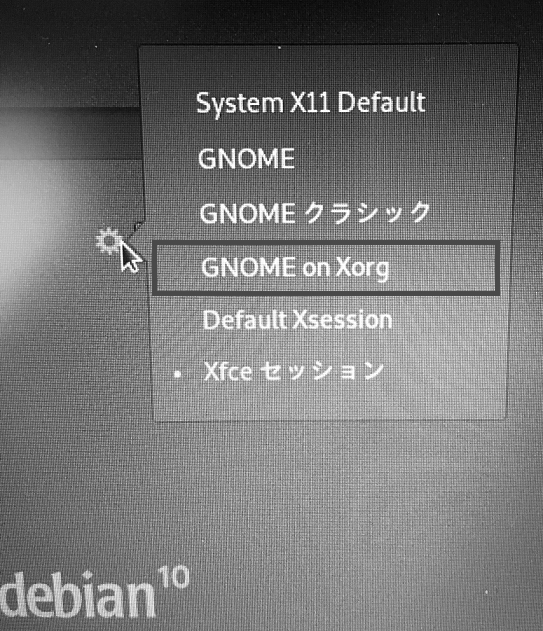
\includegraphics[width=0.5\hsize]{image201902/GDM_GNOME_select_mark_gray.png}
\end{center}



\subsubsection{新機能:/usrマージ}

新規インストールは /usr マージした状態

\begin{itemize}
  \item /\{bin,sbin,lib\} は シンボリックリンク
\end{itemize}

\begin{table}[htb]
  \begin{tabular}{|ccc|}
    \hline
    /bin  & → & /usr/bin \\ \hline
    /sbin & → & /usr/sbin \\ \hline
    /lib  & → & /usr/lib \\
    \hline
  \end{tabular}
\end{table}

\begin{itemize}
\item Debian 以外から提供されるソフトウェアを利用している場合は要注意
\end{itemize}




\subsubsection{新機能:その他}% [containsverbatim]

\begin{itemize}
\item APTへのセキュリティ強化オプションの追加
\item stableポイントリリースに対する Unattended-upgrades の挙動
\item Cryptsetup の on-disk LUKS2 への変更
\item CUPS 2.2.10 でのドライバーレス印刷機能
\item Allwinner A64 ベースのデバイスでの基本機能サポート
\item など
\end{itemize}




\subsubsection{動作の変更や制約}% [containsverbatim]

\begin{itemize}
\item glibc が新しくなり、Linuxカーネルは 3.2 以上が必要
\item Debian 9 から PostgreSQL をアップグレードした場合は DB の再インデックス化が必要
\item Wayland で動作する GNOME の一部アプリケーションに不具合がある
  \begin{itemize}
  \item 例:synaptic、fcitx
  \item Wayland で動かない場合は Xorg で動かしてみてください
  \end{itemize}
\item phpmyadmin、redmine、virtualbox などのパッケージは未収録
\item python2.7 は非推奨
  \begin{itemize}
  \item Debian 11 では削除する方向で作業中
  \end{itemize}
\end{itemize}




\subsubsection{その他の変更や制約}% [containsverbatim]

\begin{itemize}
\item OpenSSL のデフォルトが TLS 1.2 と セキュリティレベル 2
\item ブラウザ、レンダリングエンジンは Firefox ESR、Chromium、webkit2gtk のみをセキュリティサポート
  \begin{itemize}
  \item webkit や khtml エンジンを使ったwebブラウザはセキュリティサポートされない
  \end{itemize}
\item Go 関連のパッケージは制限付きのセキュリティサポート
%\item gnome-disk-utility: LUKSパスワード変更でデータ消失の危険性
\item evolution-ews は パッケージから削除
  \begin{itemize}
  \item evolution で Exchange、Office365、Outlook にアクセスができなくなる
  \end{itemize}
\end{itemize}




\subsection{バグレポート}

{バグレポートをお願いします}% [containsverbatim]
  \begin{itemize}
  \item 何かおかしい動作や不具合を見つけた場合はバグレポートをお願いします
  \item バグレポートの例 \url{https://bugs.debian.org/cgi-bin/bugreport.cgi?bug=903529}
  \item バグレポートの仕方(レポートは英語で送る必要あり)
    \begin{itemize}
    \item \url{https://www.debian.org/Bugs/Reporting.ja.html}
    \end{itemize}
  \item バグレポートの前にちょっと相談してみたい方は、日本語のDebian JPメーリングリストや、SNSで相談してみてください
    \begin{itemize}
    \item \url{https://www.debian.or.jp/community/ml/openml.html}
    \item Twitter: @debian\_jp
    \end{itemize}
  \end{itemize}


%-----------------------

\dancersection{Debian Updates}{杉本典充}

% 半年間の以下MLから抜粋して紹介する
%  debian-announce@lists.debian.org
%  debian-devel-announce@lists.debian.org


\subsection{released timeline}

{Debian Updates}% [containsverbatim]

\begin{itemize}
\item 2019/04/27:  Updated Debian 9.9  released
\item 2019/07/06:  Debian 10 released
\item 2019/09/07:  Updated Debian 10.1 released
\item 2019/09/07:  Updated Debian 9.10 released
\item 2019/09/08:  Updated Debian 9.11 released
\item 2019/11/16:  Updated Debian 10.2 released
\end{itemize}




\subsection{Bits from the DPL}

{Debian Updates}% [containsverbatim]

Bits from the DPL

\begin{itemize}
\item 月に一度の Debian Project Leader である Sam さんのプロジェクトの進捗を報告
\item 時間のない方でもこれを読んでおけば Debian Project の大まかな動きがわかる
\end{itemize}

\small{
\begin{itemize}

%\item 2018/04/30 \url{https://lists.debian.org/debian-devel-announce/2019/04/msg00010.html}
%\item 2018/06/02 \url{https://lists.debian.org/debian-devel-announce/2019/06/msg00000.html}
\item 2018/07/02 \url{https://lists.debian.org/debian-devel-announce/2019/07/msg00000.html}
\item 2018/08/12 \url{https://lists.debian.org/debian-devel-announce/2019/08/msg00001.html}
\item 2019/09/18 \url{https://lists.debian.org/debian-devel-announce/2019/09/msg00001.html}
\item 2019/10/29 \url{https://lists.debian.org/debian-devel-announce/2019/10/msg00002.html}

\end{itemize}
}




\subsection{Removal of the mips}

{Debian Updates}% [containsverbatim]

2019/08/21: Removal of the mips architecture
  
\begin{itemize}
\item mips アーキテクチャ(32bit ビッグエンディアンのmips)を testing と unstable から削除
  \begin{itemize}
  \item mips を使っている場合は mipsel または mips64el へ移行を推奨 
  \end{itemize}
\item 次の Debian 11 では mips アーキテクチャはリリースされない
\item Debian 9 および Debian 10 では mips アーキテクチャのサポートは継続
\item サポート終了の理由
  \begin{itemize}
  \item 仮想アドレス空間が 2GB までという技術的な制限
  \item 開発する人や関心を持つ人の減少
  \end{itemize}
\item 参照:\url{https://lists.debian.org/debian-devel-announce/2019/08/msg00003.html}
\end{itemize}




\subsection{Perl 5.30 transition}

{Debian Updates}% [containsverbatim]

2019/10/05: Perl 5.30 transition underway
  
\begin{itemize}
\item unstable において perl パッケージを 5.30 への切替を実施
\item 【TIPS】
  \begin{itemize}
  \item  Debian においてプログラム言語やライブラリをバージョンアップすることを「トランジション」という
  \item トランジションを行うと依存するパッケージをすべてビルドしなおす大規模な処理が行われる
  \end{itemize}
\item 参照:\url{https://lists.debian.org/debian-devel-announce/2019/10/msg00000.html}
\end{itemize}




\subsection{Python 2 removal}

{Debian Updates}% [containsverbatim]

2019/11/02: Python 2 removal in sid/bullseye: Progress and next steps
  
\begin{itemize}
\item python 2 系列は2020年1月1日にサポート終了を迎えるとアナウンスされている
\item 次の Debian 11 では python 2.7 は削除する予定
\item 進捗状況の報告、バグ報告のタグ管理方法について案内が出ている
\item 参照:\url{https://lists.debian.org/debian-devel-announce/2019/11/msg00000.html}
\end{itemize}




\subsection{Init Systems and systemd}

{Debian Update}% [containsverbatim]

2019/11/17: General Resolution: Init Systems and systemd
2019/11/20: General Resolution: Init systems and systemd: new option

\begin{itemize}
\item 今後の Init System をどうするか投票する案内が出た
\item \url{https://www.debian.org/vote/2019/vote_002}
\item 選択肢は5つ
  \begin{itemize}
  \item Init deversity is Important and NMUable
  \item Systemd but we support exploring alternatives
  \item Focus on systemd for init system and other facilities
  \item Support non-systemd systems, without blocking progress
  \item Init diversity is Required
  \end{itemize}
\item 参照:\\
  \url{https://lists.debian.org/debian-devel-announce/2019/11/msg00001.html} \\
  \url{https://lists.debian.org/debian-devel-announce/2019/11/msg00002.html}
\end{itemize}




%-----------------------

\subsection{日本語によるDebianの情報}

\begin{itemize}
  \item Debian JP Project \\
      \url{https://www.debian.or.jp}
  \item 東京エリアDebian勉強会\\
      \url{https://tokyodebian-team.pages.debian.net/}
  \item 関西Debian勉強会 \\
      \url{https://wiki.debian.org/KansaiDebianMeeting}
  \item Twitter \\
      \url{@debian_jp}
  \item 雑誌 Software Design 技術評論社発行 \\
    「Debian Hot Topics」(隔月連載)
  \item 雑誌 シェルスクリプトマガジン USP研究所発行
\end{itemize}

%\dancersection{Debian Trivia Quiz}{username}
%
%Debianの昨今の話題についてのQuizです。
%
%今回の出題範囲は\url{debian-devel-announce@lists.debian.org} や \url{debian-news@lists.debian.org}などに投稿された内容からです。
%
%\begin{multicols}{2}
%%; whizzy-master ../debianmeetingresume201211.tex
% $B0J>e$N@_Dj$r$7$F$$$k$?$a!"$3$N%U%!%$%k$G(B M-x whizzytex $B$9$k$H!"(Bwhizzytex$B$,MxMQ$G$-$^$9!#(B
%

\santaku
{DebConf13 $B$N3+:ECO$H3+:EF|$O!)(B}
{$BF|K\!"El5~ET(B 6$B7n(B20$BF|(B}
{$B%K%+%i%0%"(B $B%^%J%0%"(B 7$B7n(B8-14$BF|(B}
{$B%9%$%9!"%t%)!<%^%k%-%e(B 8$B7n(B11-18$BF|(B}
{3}
{$B%K%+%i%0%"$O(BDebConf12$B$N3+:ECO$G$9!#(B
DebConf13$B$O%9%$%9$N%-%c%s%WCO$G3+:E$G$9!#(B
6/20$B$O3'$5$sM=Dj$r6u$1$F$*$-$^$7$g$&!#(B}

\santaku
{$B@$3&$N(BWeb$B%5!<%P$G:G$b?M5$$N$"$k(BLinux $B%G%#%9%H%j%S%e!<%7%g%s(B(W3Techs$BD4$Y(B)$B$O!)(B}
{CentOS}
{Debian}
{Ubuntu}
{B}
{\url{http://w3techs.com/technologies/history_details/os-linux}$B$K7k2L$N%0%i%U$,$"$j$^$9!#(B
$B8=:_(B Linux $B$r;HMQ$7$F$$$k(B web $B%5!<%P$N(B 32.9\% $B$,(B Debian $B$rMxMQ$7$F$*$j!"$=$N3d9g$O8=:_$bA}2C$rB3$1$F$$$k$=$&$G$9!#(B}

\santaku
{Debian $B%+!<%M%k%A!<%`$N%a%s%P!<$G$"$j!"(Bkernel.org $B$N(B 3.2.y $B0BDjHG7ONs$N%a%s%F%J$G$b$"$k(B Ben Hutchings $B$5$s$,<!4|(B Debian $B0BDjHG$H0l=o$K=P2Y$5$l$k(B Linux $B%+!<%M%k$K(B (3.2 $B7ONs$N(B mainline $B$K$OL5$$(B) $BDI2C5!G=$,Ek:\$5$l$kM=Dj$G$"$k$H=R$Y$F$$$^$9!#(B
$BB?$/$NDI2CE@$NCf$K4^$^$l$J$$$b$N$O2?!)(B}
{PREEMPT\_RT}
{Hyper-V guest drivers$B$N6/2=(B}
{ARM64/AArch64$B%"!<%-%F%/%A%c%5%]!<%H(B}
{C}
{Hyper-V guest drivers$B$O(Bmainline kernel$B$G(B3.2$B$K$b4^$^$l$F$$$^$9$,!"$h$j2~A1$5$l$?(B3.4$B$+$i$N=$@5$,F3F~$5$l$^$9!#(B
PREEMPT\_RT$B$O%O!<%I%j%"%k%?%$%`$r<B8=$9$k$?$a$N(BPatch$B!"(B
linux-image-rt-amd64 , linux-image-rt-686-pae $B$N(Bmetapackage$B$G;HMQ$G$-$^$9!#(B
$B?7$7$$(BARM 64$B%S%C%H%"!<%-%F%/%A%c%5%]!<%H$O(Bmainline kernel 3.7$B$+$i(B}

\santaku
{Wookey$B$5$s$,%"%J%&%s%9$7$?(Balpha$BHG$N(BDebian port arm64 image$B$O!)(B}
{Debian/Ubuntu port image}
{Debian/KFreeBSD port image}
{Debian/GnuHurd port image}
{A}
{self-bootstrapp(non x86)$BBP1~$H$N$3$H$G$9!#(B\url{http://wiki.debian.org/Arm64Port}$B$G%9%F!<%?%9$,3NG'$G$-$^$9!#(B}

\santaku
{700,000$BHVL\$N%P%0$,Js9p$5$l$?F|$rEv$F$k(B700000thBugContest$B$N7k2L$,=P$^$7$?!#$=$NM=A[F|$HJs9pF|$O!)(B}
{2012/12/12$B$rM=A[$7$?(BDavidPrevot}
{$BM=A[F|(B:2013/02/04$B!"Js9pF|(B:2013/02/14}
{$BM=A[F|(B:2013/02/07$B!"Js9pF|(B:2013/02/14}
{$BM=A[F|(B:2013/02/14$B!"Js9pF|(B:2013/02/07}
{C}
{$B:G$b6a$$(B2013/02/14$B$rM=A[$7$?(BChristian Perrier$B$5$s$,Ev$F$^$7$?!#7k2L$O(B\url{http://wiki.debian.org/700000thBugContest}$B$G8x3+$5$l$F$$$^$9!#(B
$B$^$?!"(B800,000/1,000,000$BHVL\$N%P%0$,Js9p$5$l$kF|$rEv$F$k%3%s%F%9%H(B\url{http://wiki.debian.org/800000thBugContest}$B$b3+:E$5$l$F$$$^$9!#(B}

\santaku
{master.debian.org$B$,?7$7$$5!3#$K0\9T$5$l$^$7$?!#$3$l$O2?$N%5!<%P$G$7$g$&$+(B $B!)(B}
{@debian.org$B$N%a!<%k%5!<%P(B}
{$B%Q%C%1!<%8$N%^%9%?!<%5!<%P(B}
{$B%Q%C%1!<%8$N%9%]%s%5!<(B(mentor)$B$rC5$9%5!<%P(B}
{A}
{$B8E$$%5!<%P$O%G%#%9%/>c32Ey$,$"$C$?$N$G!"<wL?$HH=CG$5$l!"%G!<%?$,B;<:$9$kA0$K?7$7$$%5!<%P$K0\9T$5$l$^$7$?!#(Bftp-master.debian.org$B$O(BDebian$B$N(B official package $B%j%]%8%H%j$G$9!#%Q%C%1!<%8$N%9%]%s%5!<(B(mentor)$B$rC5$9$N$O(Bmentors.debian.net$B!#(B }

\santaku
{pbuilder$B$K(Bclang support$B$,DI2C$5$l$^$7$?!#C/$,=q$$$?%Q%C%A$G$7$g$&$+!)(B}
{Sylvestre Ledru}
{Junichi Uekawa}
{Hideki Yamane}
{C}
{Debian$B$N(BClang$B%5%]!<%H$OCe!9$H?J$s$G$$$^$9!#(B}

\santaku
{DPN - 2013$BG/(B3$B7n(B4$BF|9f$K<h$j>e$2$i$l$?F|K\$N%$%Y%s%H$O(B}
{Open Source Conference 2013 Tokyo/Spring}
{Open Source Conference 2013 Hamamatu}
{Open Source Conference 2013 Tokushima}
{A}
{\url{http://henrich-on-debian.blogspot.jp/2013/02/open-source-conference-2013-tokyospring.html} $B>\:Y$O8e$[$I!#(B}


%\end{multicols}


% % (query-replace-regexp "<.*?>" "")
% % (query-replace-regexp "^[    ]\+" "")

\dancersection{\mbox{自作キーボード温泉に}\mbox{日帰り入浴してみた話}}{小林 克希}

\subsection{はじめに}

みなさん、キーボードは何をお使いでしょうか?
この記事では、最近巷で流行っているという「自作キーボード」について、
私が実際に作ってみたり、その後色々と調べたりした内容について話そうかと思います。
そもそも何故私がキーボードを自作してみようかと思ったか、ですが、
要は肩凝りと腰痛がひどかったから……だったりします。
とくにここ2年間くらい、仕事中に腰が悲鳴をあげ、
じっと席に座っていられないという状況に陥っており、
フィットネスクラブにも通い、整骨院にも通い……としましたが、全然改善せず大変に悩んでおりました。

そんな中思い至ったのがキーボードでした。
私は、5年ほど前に初めてThinkpadを購入したのですが、トラックポイントがいたく気にいり、
デスクトップ用のキーボードについてもThinkpadキーボードに乗り換えました。
ご存知の方も多いとは思うのですが、このThinkpadキーボード、
常にホームポジションから手をはなさずにいられるという点は大変にすばらしいのですが、
トラックポイントって、結構操作に力が入るのですよね……。
細かいカーソル操作をしている場合なんか特に。

ということで、一度他のキーボードを試してみるか……と思い至り、
最初は市販の分割キーボードのUltimate Hacking Keyboard%
\footnote{\url{https://ultimatehackingkeyboard.com/}}
がトラックポイントも付けられるみたいだしよさそう、と思ったのですが、
金額的にも、納期的にも、触ってもないのに手を出すのはどうかなぁ……と尻込みし、
\textbf{結局自作することにしました}。
なにを言ってるんだこいつはと思うかもしれませんが、
関西Debian勉強会メンバーのKさんの親指Ctrlの布教が功を奏したとでも思ってください。

ところで、自作キーボードといっても、作成具合にレベルがあるようなのですが、
一番基本的な自作方法は、キーボードキットを購入し、
別途キースイッチやキーキャップも好みのものを購入していく形になるかと思います。
わたしも、今のところはキットを購入して作成したので、
今回はそのあたりの流れをご紹介できればと思います。
\textbf{「Debian関係あるのか?」}、ですって?
{\scriptsize ……………………ほとんどありません……} のちほど、
気持ちだけ出てきます……。

なお、この文章は関西Debian勉強会の2019年11月に発表した内容であるため、
\footnote{\url{https://speakerdeck.com/rarewin/self-made-keyboard}}{スライド}
の方もご参照いただければと思います。

\subsection{キーの数と配列}

さて、実際にキーボードの自作をするという気になったはいいものの、
はたしてどういったものがよいのか困るかと思います。
そんな中でも、一番気になるのは配列ではないでしょうか。
ということで、まずはどんな配列があるのかについて簡単に説明をしていこうかと思います。
ところで、自分の追い求めた理想のキーボードのことを、この業界の人達は \textbf{Endgame} と呼ぶそうです。
アベンジャーズ?

\subsubsection*{XX\%キーボード}

まず、キーの個数が重要な気がします。
キーの個数については、フルキーの104キーに対して、そのキーボードのキーの数をパーセンテージであらわすのが
一般的なようです。
主流のものとしては、テンキー・ファンクションキーあたりを省いたものが
60\%(HappyHackingKeyboardあたりがこのサイズになります。)、
そこからさらにフルキーから数字の段を除いたものが40\%となるようです。

なお、逆に、100\%を越えるようなキーボードもあり、
たとえば左側にもテンキーがあったりするものがあるようです。
どちらかというと、ゲーム用な感じでしょうか。
あと、全てのemojiが打てるキーボード%
\footnote{\url{https://thenextweb.com/insider/2015/09/22/say-goodbye-to-words-the-emoji-keyboard-is-real/}}
だとか
10\%切ってるようなイカれたキーボード%
\footnote{\url{https://www.reddit.com/r/MechanicalKeyboards/comments/dnrvz8/science_isnt_about_why_its_about_why_not/}}。
もあるようです

\subsubsection*{キーの物理配列}

キーの個数と同時に考えないといけないのが配列です。
配列……というとQWERTYとかDvorakとかの論理配列かが思いおこされるかと思いますが、
自作キーボードでは、論理配列はファームウェアをいじれば自由自在であるため、
この界隈で配列といったら物理的な配列のことを指すような気がします。

ところで、物理的な配列で思い起こされるのは、市販されてるキーボードとしては、Microsoftなどが出してる、
いわゆる「エルゴノミクスキーボード」と呼ばれるような
「G」と「H」の間あたりに隙間が空き、「G」や「H」よりも「A」や「;」が奥の方に配置されているものではないでしょうか。
自作キーボード界ではもっと極端に、完全に分割している分割キーボードが流行っています(特に日本で、のようです)。
なお、分割はしてますが、基本的には両者の間にシリアル通信用のケーブルを這わすので、
ちゃんと両者は連携できます。

また、分割しているだけではなく、キーのズレ方にもいくつか種類があります。
まず、普段みかける、いわゆる「普通の」キーボードのように、
行ごとに左右に少しずつずれている配置については「row-staggered」、
もしくは「normal-staggered」と呼ばれます。
対して、列ごと、すなわち「QAZ」は綺麗に縦に揃っているが、
各列はずれている配列の事を「column-staggered」と呼びます。
ぱっと見ると、「この配列は使えるんだろうか……」とか思うのですが、
コンセプトとしては、指の長さに合わせて各列の位置を調整できるのが嬉しいようです。
さらには、ひたすらコンパクトさを求め、完全に格子状に並べた
直交配列とかOrtholinearとか呼ばれるものもあります。
また、逆にキーボードのサイズが大きくなるのはお構いなしに、
指の形状による配列を追い求めまくったTRONキーボードとかもあります(が、こちらのキットはみかけないかな……)。

\subsection{各パーツ}

つぎに、自作キーボードにおいて必要となる各種パーツについて簡単に解説していきます。
なお、2019年12月現在では、実店舗のある自作キーボード専門のお店は、
秋葉原にある遊舎工房さん\footnote{\url{https://yushakobo.jp/}}のみのようです。
なお、関西はどうなっているかというと、
日本橋のシリコンハウス\footnote{\url{http://silicon.kyohritsu.com/}}にて、
最近になってキットや、CherryとGateronのキースイッチの販売が開始されたり、
自作キーボード組み立てのワークショップが行なわれたりと、確実に風は吹いてきている!!……ようです。
あ、日本橋の千石電商\footnote{\url{https://www.sengoku.co.jp/shop_osaka.html}}でも、
KailhとCherryのキースイッチがあるようでした。

\subsubsection*{キースイッチ}

キースイッチには色々と方式があったりするようですが、
実際にキーボードを自作しようとすると、
流通や、各基板(PCB)の対応といった観点から

\begin{itemize}
 \item Cherry MX
 \item Kailh Choc (通称、Kailhロープロファイル)
\end{itemize}

の二種類のメカニカルキースイッチを使う事になると思います。
前者は、ドイツ企業のCHERRY社が出しているキースイッチで、
特許が切れているため他のメーカーが互換品を出しており、
たぶん一番種類が豊富なキースイッチかと思います。
そのため、世間一般で販売されているような自作キーボードキットの
ほとんどの基板はこちらのスイッチに対応しているかと思います。
手元にあるこのタイプのスイッチの写真を図\ref{fig:cherry-compat}に置いてみます。
互換品なので当然ですが、ぱっと見た感じではみんな同じ形をしています。
打鍵具合や値段もかなりピンキリなので、色々と見てると楽しいかと思います。

\begin{figure}[htbp]
 \begin{center}
  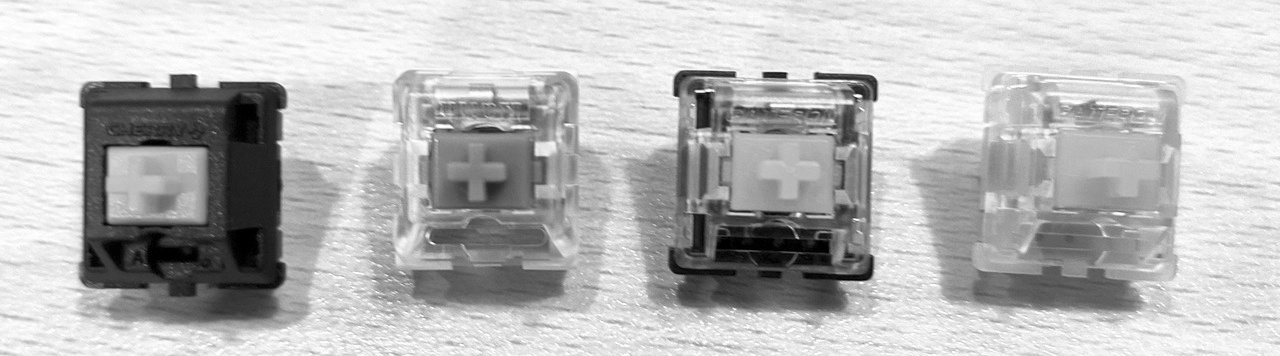
\includegraphics[keepaspectratio,height=2cm]{./image201911-kansai-02/cherry-compat.jpg}
 \end{center}
 \vspace*{-1zw}
 \caption{左から順に、Cherry MX(Red)、Kailh Speed(Copper)、Gateron MX(Red), Gateron MX Silent(Red)}
 \label{fig:cherry-compat}
\end{figure}

また、最近流行ってきているのが後者のKailhロープロファイルと呼ばれる、かなり薄い感じのキースイッチです。
図\ref{fig:helix-katsu}にあるのが、私が今使用しているHelixというキーボードの左手側の部分なのですが、
ずいぶんと薄くてコンパクトな感じになるキーになります。
ただし、注意点として、CherryMXとKailhロープロファイルについては、基板に互換性がないため、
基板が対応していない場合は使うことができません。
それでも、両方のスイッチに対応した設計になっている基板も存在するので、
基板選定の際には、どのスイッチに対応しているのか確認が重要です。

\begin{figure}[htbp]
 \begin{center}
  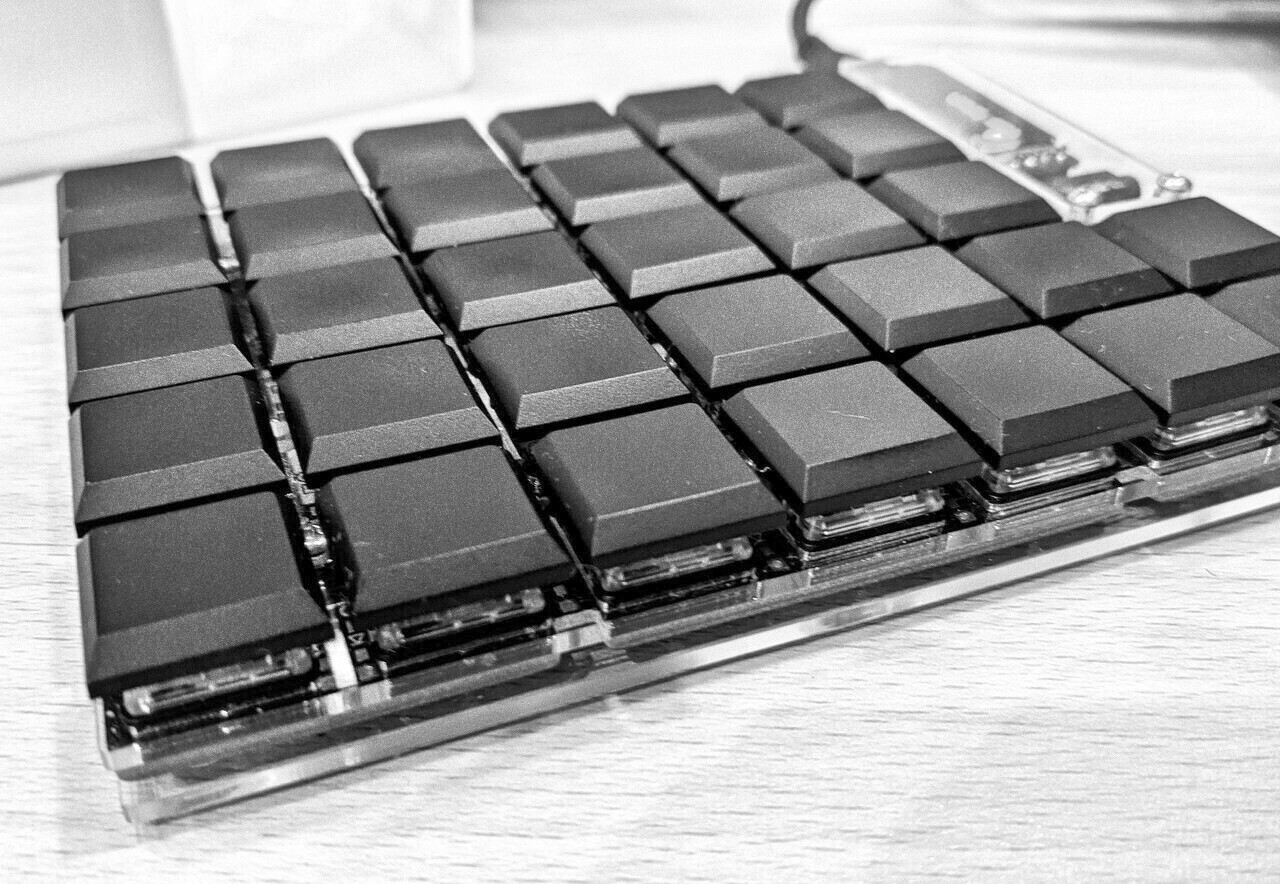
\includegraphics[keepaspectratio,width=5cm]{./image201911-kansai-02/helix.jpg}
 \end{center}
 \vspace*{-1zw}
 \caption{Helixキーボード(左手)}
 \label{fig:helix-katsu}
\end{figure}

で、打鍵感的なものについては、いわゆる「軸」というやつが関係していて、
CherryMXについては
色によって表\ref{tab:cherry-jiku}のような特徴があります。
余談ですが、2019年12月現在、梅田ヨドバシのキーボード売り場には
Cherryのキースイッチのテスターが置いてありますので、興味あれば直接さわってみてはいかがでしょうか。
この間行ったときは、ずいぶんとわかりづらいところに引っこんでしまっていましたが。

また、互換スイッチでも、だいたいCherryの同色の軸と同じような性能になってますが、
たまに性能的に全然違うものや、Cherryには無い色(Gateronの黄色いのとか、Kailhの紫色だとか)とかもあったりするので、
購入前には、実物を触るのが一番良いですかね。
それができなくても、スペックシートを見たり、どっかのブログを見たりするのが良いと思います。
Kailhのロープロファイルについても、流通しているもので赤軸・白軸・茶軸と3種類あります。
メーカーのサイト\footnote{\url{http://www.kailh.com/en/Products/Ks/CS/}}を見てると
他の軸もあるようなので、そのうち選択肢が広がるかもしれません。

\begin{table}[htbp]
 \begin{center}
  \caption{Cherry MXの軸ごとの特徴}
  \label{tab:cherry-jiku}
  \footnotesize
  \begin{tabular}[tb]{c|cccc}
   \hline
   軸       & クリック感 & 音       & 重さ   & 深さ \\ \hline \hline
   ピンク軸 & なし       & しずか   & かるめ\\
   赤軸     & なし       & ふつう   & かるめ\\
   茶軸     & あり       & ふつう   & ふつう\\
   黒軸     & なし       & ふつう   & おもめ \\
   青軸     & あり       & カチカチ & おもめ \\
   銀軸     &            &          &        & 浅め \\ \hline
  \end{tabular}
 \end{center}
 \begin{flushright}
  {\footnotesize 参考: \url{https://www.diatec.co.jp/products/CHERRY/}}
 \end{flushright}
\end{table}

他にメジャーどころとして、ALPSというキーもあるみたいなのですが、
現在は純正品は生産が停止されているそうです。
根強い人気のようで、キットだけ販売されてたりするようですが……。
また、ロープロファイルについてはCherryのロープロファイルもあったり、
KailhもChocよりもさらに薄いX Switchと呼ばれるものがあったりするようですが、
遊舎工房さんとかでもまだ扱ってないので、
いまのところ、イベントでその手の方のを触らせてもらうか、
それらのキーを使用している市販キーボード(高級)を買うかしかなさそうです。
なお、キースイッチについてですが、
ピンソケットを付けて、後から付け換えできるようにすることもできます。
基板が対応していたら、キースイッチ専用のものを、
していなくても、汎用のピンソケットをつかって対応している人もいるようです。

\subsubsection*{キーキャップ}

次に重要なパーツとして、キーキャップがあります。
まず、形(プロファイル)について、DCSとかDSAとか色々あって、
平たい部分の面積が違ったり、角度が違ったりと色々とあるようです。
が、私はまだこのあたり、くわしくないのであまりちゃんと説明できません……。
キーキャップセットだけでも結構なお値段ですので!!

ただ、注意点としては、キーのサイズとしては普通のアルファベットのキーを1Uとして、
0.25刻みで1.25U、1.5U……といったぐあいのキーサイズが存在しています。
少々ややこしいのが、キットによってキーのサイズが異なることです。
たとえば、図\ref{fig:helix-katsu}のHelixの場合、シフトキーやコントロールキー、
全てが1Uになってるようなものもあれば、
シフトキーやスペースキーは2U以上のサイズのキーであるようなものもあります。
これの何がややこしいかというと、キーキャップとキーボードでキーのサイズが一致しないと、
刻印が異なるキーを付けざるを得ない状況が発生するのです。
たとえば、この後紹介しますが、私の利用しているMint60というキーボードについては、
スペースキーが2つに分割されたような配列なのですが、
一緒に販売されていたキーキャップセットでは
そのサイズのスペースキーがなく、代わりにシフトキーを被せています。
そして、シフトキーの位置には、テンキーの0が挿さっていたりします。

\subsubsection*{マイコン(ProMicro)}

元々はSparcFun社が出しているマイコンボードで、Arduinoの開発環境が使えるボードです。
サイズが小さく、ピンもそこそこあり、かなり使い勝手の良いボードなんですが、
定価だと2,500円くらいとちょっとお高いです。
が、今では色々なクローンができて、それらが大変おやすく(500円とか)手に入るため、
キーボード用ファームウェアの環境も整備されたことも手伝い、
こちらのボードがこの界隈では標準になっているようです。

ただ、このマイコンボード、いくつか問題もありまして、
一番大きいのはUSBのソケットがMicro-Bで、そのソケットももげやすいというおまけ付きです。
そのため、エポキシ接着剤で補強したり、ソケット強化版とかType-C版のProMicroも販売されていたりします。
また、そもそも無線キーボードじゃないと嫌だという人向けに
BLEを積んだProMicroも販売されています。
が、それらは結構な値段で販売されているため、微妙と言えば微妙……。
それを嫌って、他のマイコンボードを使うキーボードもいくつかあります。

\subsubsection*{OLED/LED}

また、キーボードと直接関係あるような無いようなですが、
自作キーボードキットにはOLEDのディスプレイやLEDが付属するものが多いです。
前者は、キーのレイヤー表示に使われたり、キットのロゴを表示させる等色々に使われています。
LEDに関しては完全に趣味ですね……。
キーボードはカッコよく光るべきものらしいです。
LEDには、表面側を照らすBacklight型と、底面側を照らすUnderflow型の二種類があります。

で、気をつけたいのが、LEDがチップタイプのものを用いるキットです。
このチップタイプのもの、小さい上に熱に弱いので、
これがあるキットというだけではんだ付け難易度が跳ね上がります。
特にHelix系のキーボードは、本来LEDチップが想定している方法とは異なる方法で実装するため、
ある程度はんだ付けに慣れてる人でないと難しいかもしれません。
とは言え、光らすと図\ref{fig:helix-katsu-lightning}のように、
なかなかに爽快な感じになるので、格好よさを求めるのであれば、是非挑戦していただきたいところです。

\begin{figure}[htbp]
 \begin{center}
  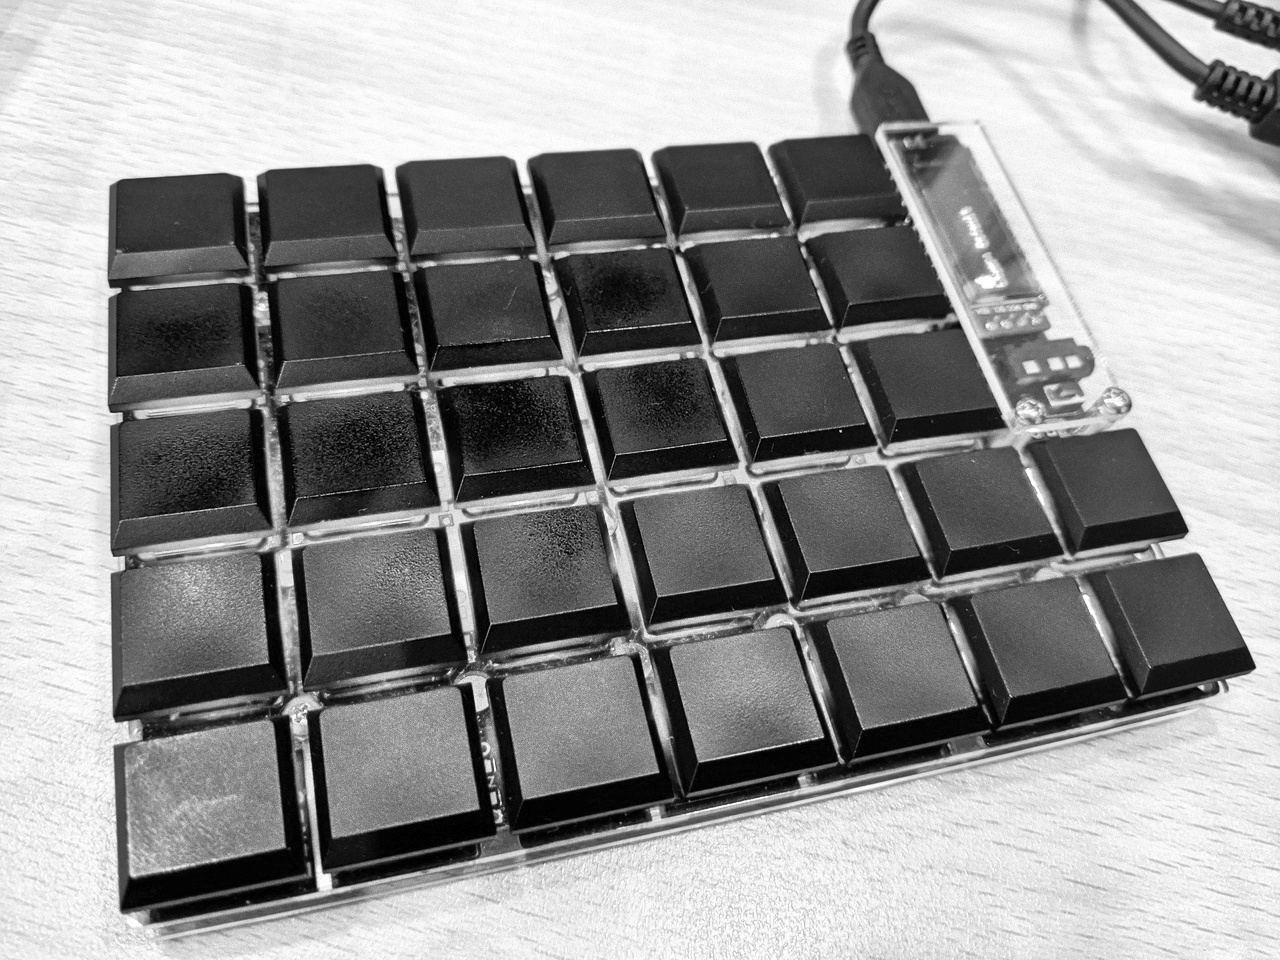
\includegraphics[keepaspectratio,width=5cm]{./image201911-kansai-02/helix-lightning.jpg}
  \hspace*{2zw}
  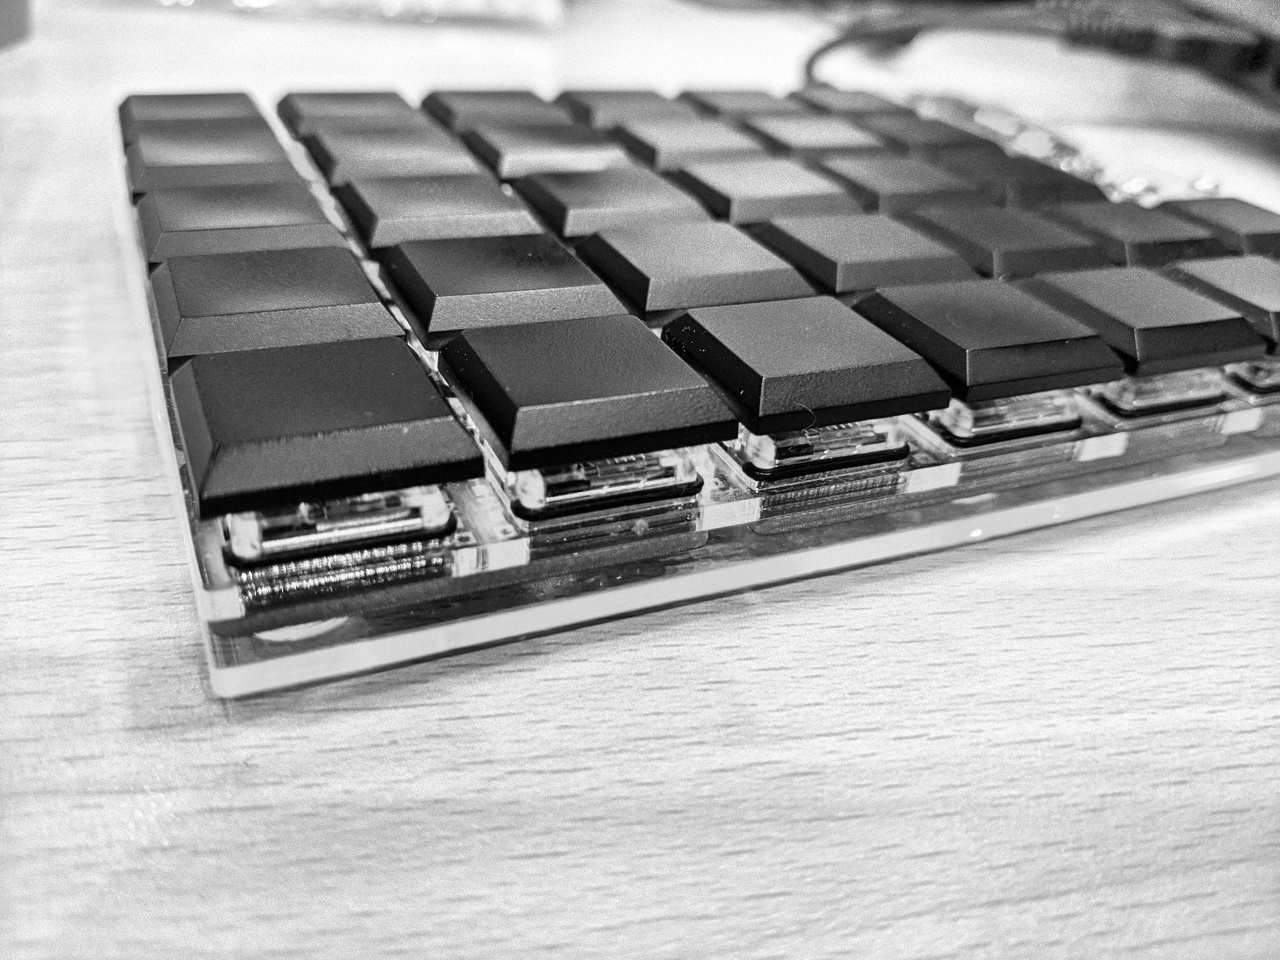
\includegraphics[keepaspectratio,width=5cm]{./image201911-kansai-02/helix-lightning2.jpg}
 \end{center}
 \vspace*{-1zw}
 \caption{Helixキーボード(左手)を光らせたところ(カラーでないのが残念!!)}
 \label{fig:helix-katsu-lightning}
\end{figure}

\subsection{キットの選定・購入}

ということで、ここまでの話を考慮した上でキットを選んでいくのですが、
国内でキットを購入しようとした場合、おそらく遊舎工房さん、
もしくはBOOTH\footnote{\url{https://booth.pm/ja}}で購入する流れになるかと思います。
他の手段ですと、キットを取り扱っている電子工作パーツ店をみつけたり、
キーボード関連のミートアップ等の即売会に参加することになると思います。

キットによっては、ダイオードとしてSMDタイプとよばれるすごく小さいものが
付いてきたりします。私が組んだHelixなんかはそうでした。
こちらは、足が小さいためはんだ付け難易度は高いかと思います。
ただ、実はHelixやその派生キーボードは、SMDタイプよりもはんだ付け難易度の低い
足の付いた素子のタイプのダイオードも使えるようになっていますので、
別途購入が必要ですが、たいした金額ではない(数百円程度)ので、
欲しいキットがあってもはんだ付けに自信がなければ、
そのような事ができないかを確認されても良いかもしれません。

また、やはり一番気になるのはキーの物理的な配列かと思います。
キーの個数だとか、物理配列だとか、「そんな普通と違うようなキーボード打てる気がしない」
とおっしゃる方もおられるかもしれません。
\textbf{実際、その通りでございまして、}
私のまわりで、キーが少な目で、column-staggeredなキーボードを作成した二人は、
「打つのにストレスが溜まる」と言い出して、そのキーボードをつかうのを諦めてしまったようです。
ということで、各位におかれましては、
いきなり奇抜なものとかEndgameを狙わずに、\textbf{初めは}普段使っているキーボードに近い形の
自作キーボードに手を出す事を強くお勧めします。

%ここでは、私が使っている「Mint60」と「Helix」について紹介していきます。
%
%\subsubsection*{Mint60}
%
%私が一番最初に組んだキーボードです。
%\subsubsection*{Helix}

\subsection{キットの組み立て}

キットを購入したら、当然組み立てが必要です。
必須なものとしては
「はんだ」「はんだごて」「はんだごて台」と「ドライバー」あたりでしょうか。
「はんだ」は、無理して鉛フリーとかは止めといた方がよいと思います。
また、「はんだごて」は温度の調整が可能なもの(比較的安めのものもあります)、
「はんだごて台」の汚れ落としは、水を使うのではなく、金色の金たわしみたいなやつ%
\footnote{会社の人は「ゴールデンアフロ」と呼んでいました。}
の方が温度が下がらなくてオススメです。
キーボードを作るのに必要なはんだ付けは、大抵そんなに難易度の高いものはないので、
無理して高い物を買う必要はありませんが、
この辺りの装備は、あまり安い物を買うと後で後悔するかもしれません。

また、実際には「ラジオペンチ」「ニッパー」「ピンセット」もあった方が良いですし
(素子タイプのダイオードならニッパーは必須)、
「テスター」や「はんだ吸いとり器」もしくは「はんだ吸い取り線」は準備した方が良いと思います。
特にテスターについては、キーボードを作るとダイオードとキースイッチのはんだ付けでも100箇所以上となるので、
大体どこかが接触不良だったりしますし、
方向間違えたり、チップを壊したりとかもありますので、安めのものでもあった方が良いかと思います。

なお、キットですが、基本的には「基板」「ケース」「マイコンボード」に加えて
スイッチやケーブルのコネクタなどの小物あたりがセットになって販売されており、
「キースイッチ」「キーキャップ」およびケーブル類は別売りになっている事が多いです。
そこは、自分で好きに選んでくれという話なのかと思います。
また、キットによってはケースとPCBが別売りになっていることがあります。
これは、ケースがアクリル以外にもステンレス製のものがあるキットもありますし、
遊舎工房さんが、メジャーなキットについては
ケースの色を選んで作ってくれるサービスをはじめたから、というのもありそうです。
LEDとかOLEDが別売りであるキットもありますので、
キット購入の際は、付けたいものが揃っているか確認するのをおすすめします。

\subsubsection*{Mint60の場合}

私が最初に作ったMint60の場合、キーキャップやキースイッチもセットで販売してくれていますので、
私の場合は素直にそれらコミコミのセットで注文しました。
届いて開封したときの写真を図\ref{fig:mint60-katsu-unpack}に掲載してみました。

\begin{figure}[htbp]
 \begin{center}
  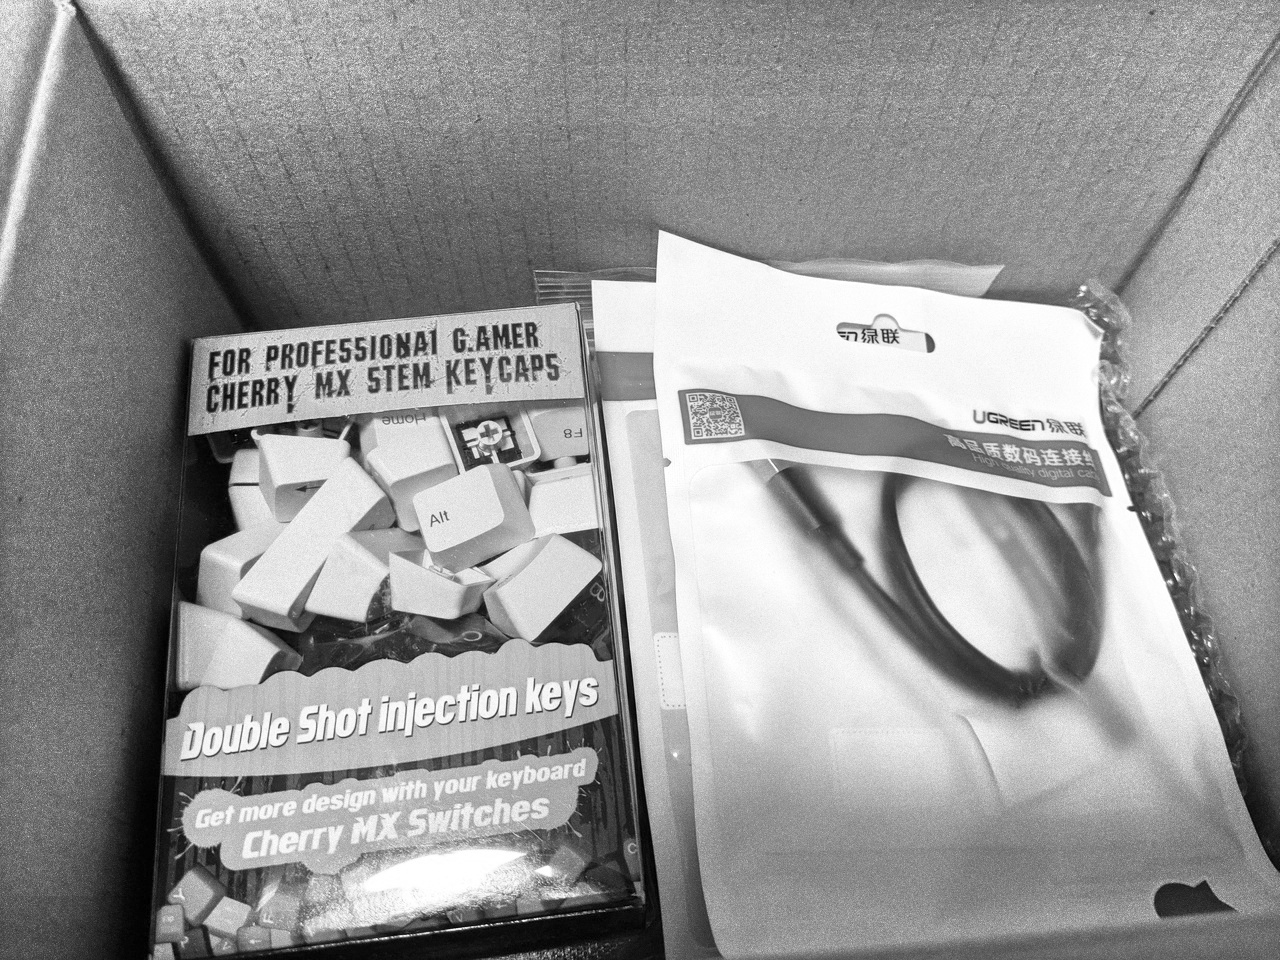
\includegraphics[keepaspectratio,width=5cm]{./image201911-kansai-02/mint60-unpack-01.jpg}
  \hspace*{2zw}
  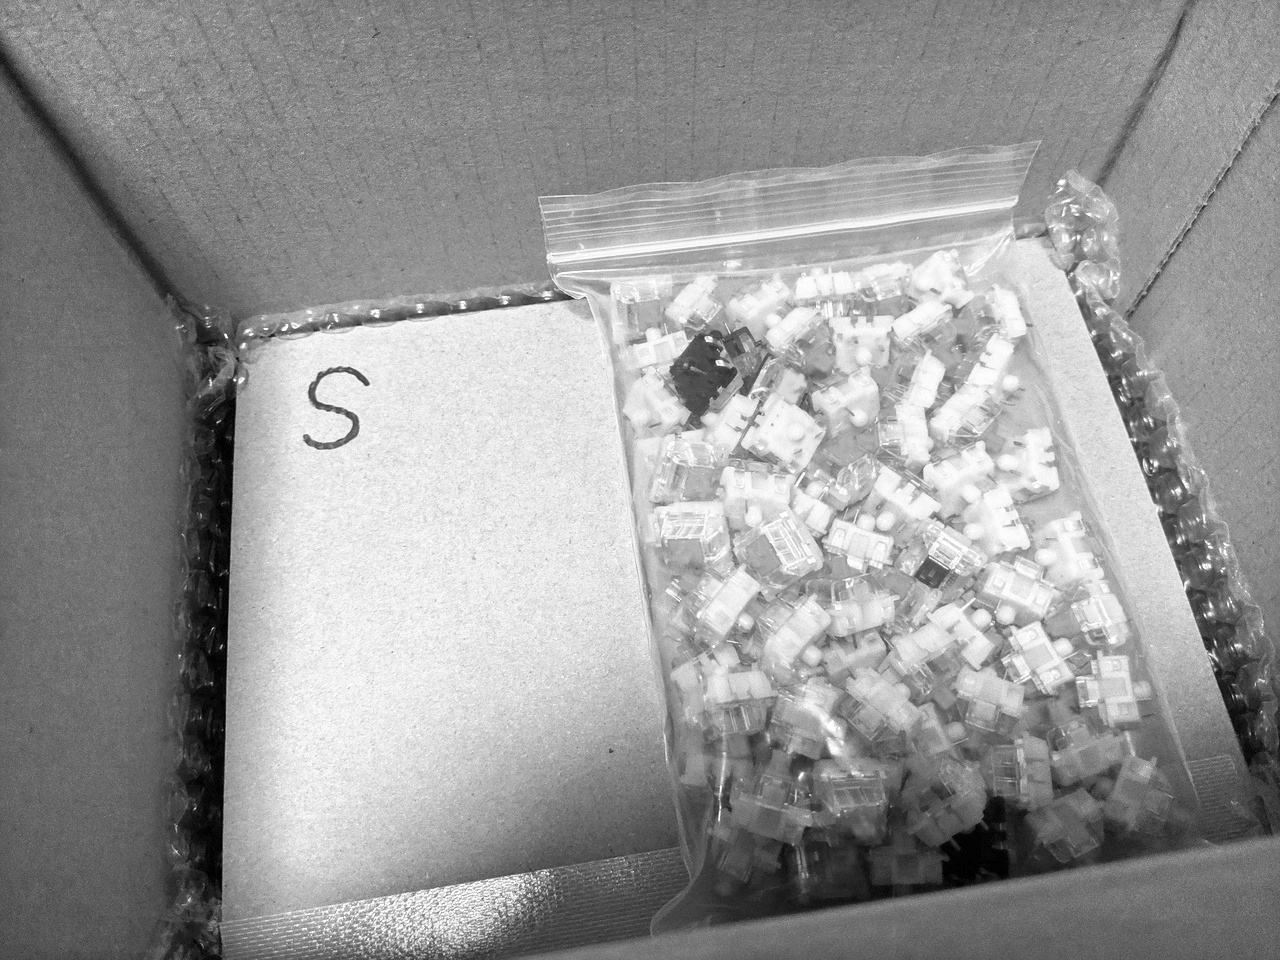
\includegraphics[keepaspectratio,width=5cm]{./image201911-kansai-02/mint60-unpack-02.jpg}
  \hspace*{2zw}
  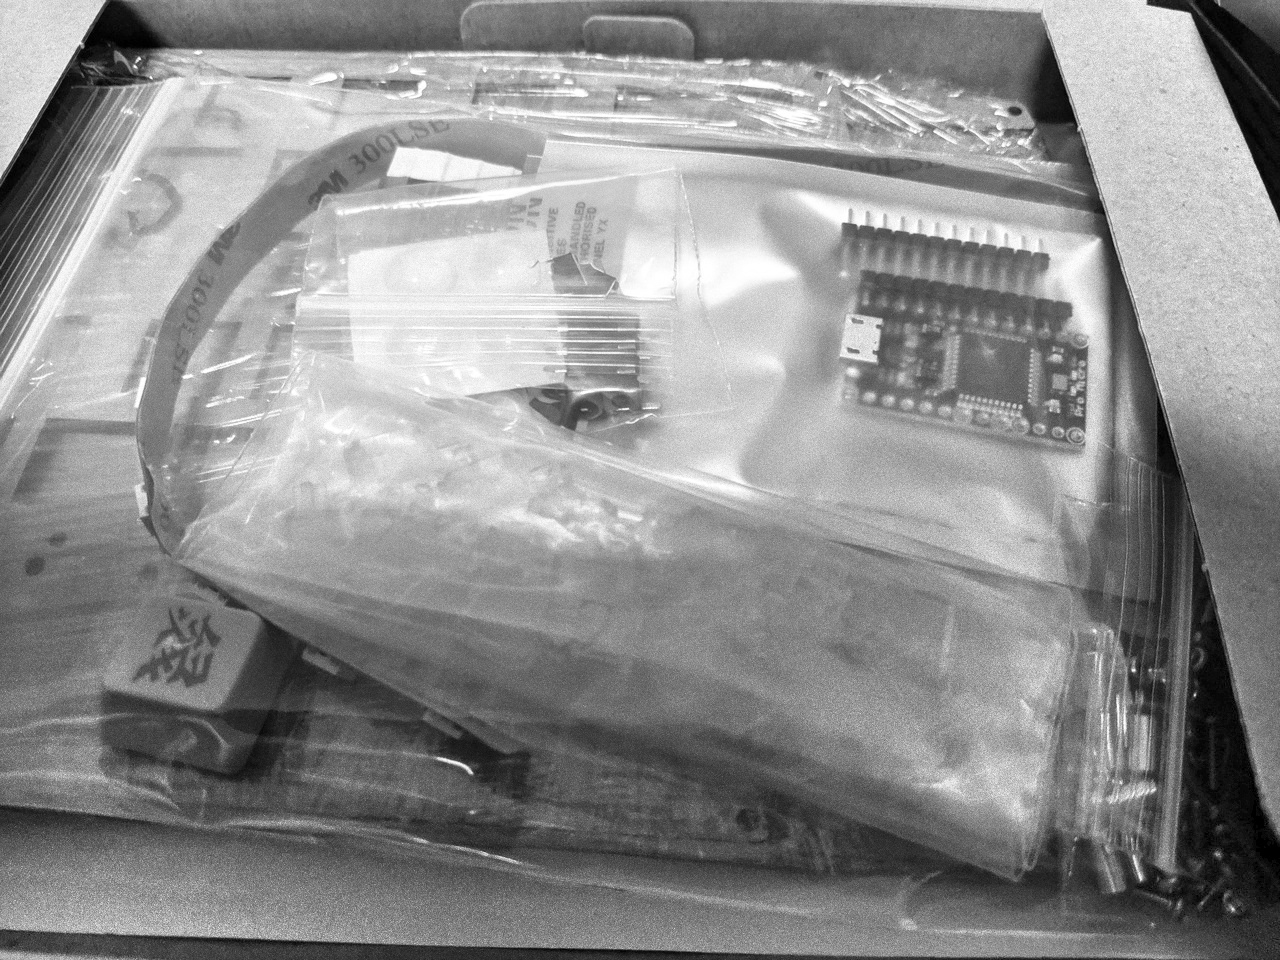
\includegraphics[keepaspectratio,width=5cm]{./image201911-kansai-02/mint60-unpack-03.jpg}
 \end{center}
 \vspace*{-1zw}
 \caption{Mint60開封の儀}
 \label{fig:mint60-katsu-unpack}
\end{figure}

これを、図\ref{fig:mint60-katsu-build}のように、リセットスイッチや
通信用のケーブルのジャックや、ProMicro、ダイオード、キースイッチをはんだ付けしていくだけです。
なお、一番右の図でPCBにキースイッチだけ生えてますが、
\textbf{実はこれは失敗例で、間にアクリルのカバーを挟んで実装するのが正解です。気をつけましょう。}
間違えると、泣きながらはんだ吸い取り器をAmazonでポチり、
キースイッチ全てとProMicroを嗚咽しながら剥ぎ取るという不毛な作業が必要になります……。

\begin{figure}[htbp]
 \begin{center}
  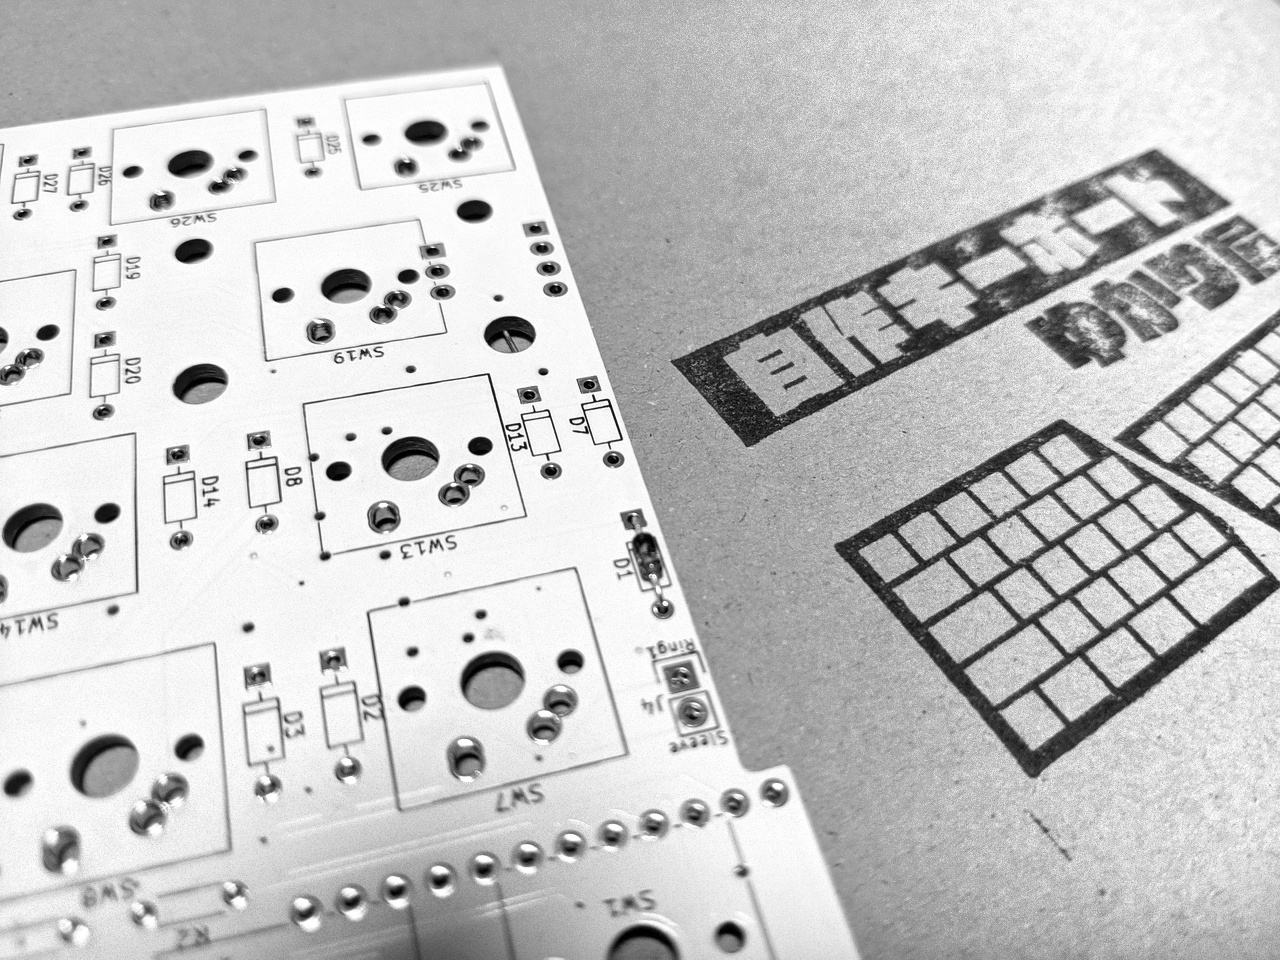
\includegraphics[keepaspectratio,width=5cm]{./image201911-kansai-02/mint60-build-01.jpg}
  \hspace*{2zw}
  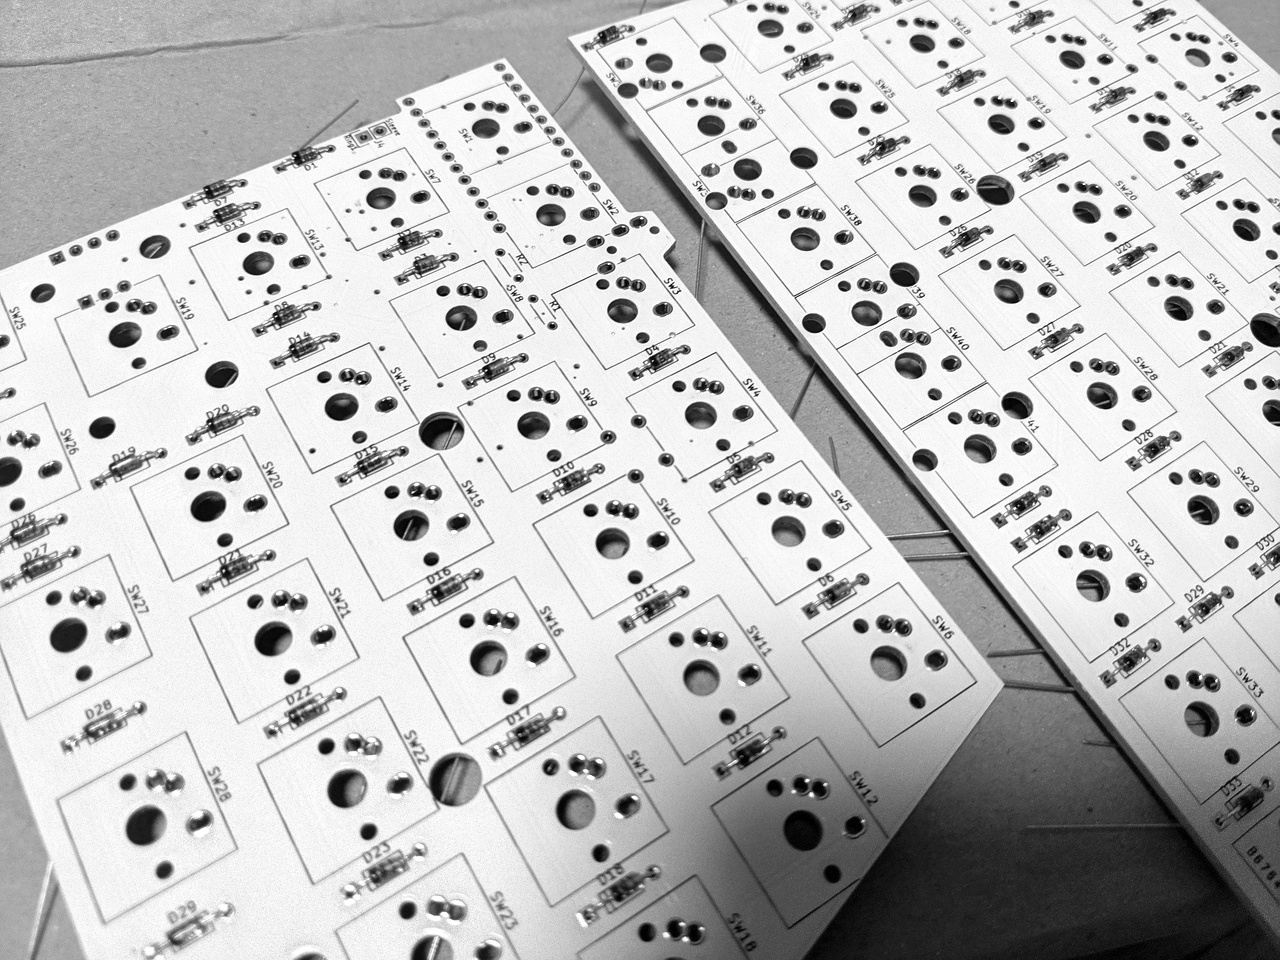
\includegraphics[keepaspectratio,width=5cm]{./image201911-kansai-02/mint60-build-02.jpg}
  \hspace*{2zw}
  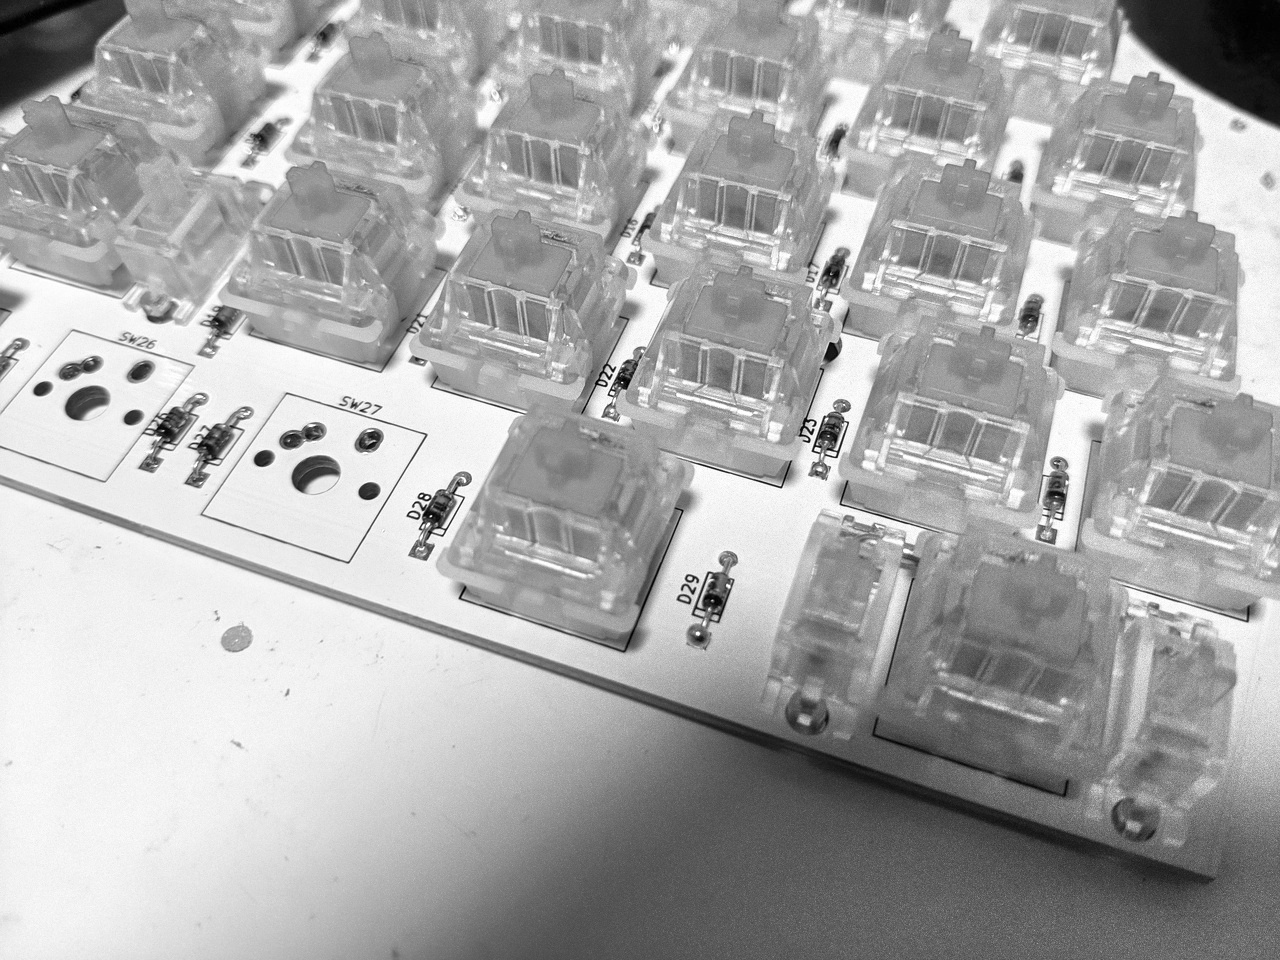
\includegraphics[keepaspectratio,width=5cm]{./image201911-kansai-02/mint60-build-03.jpg}
 \end{center}
 \vspace*{-1zw}
 \caption{Mint60 組み立て}
 \label{fig:mint60-katsu-build}
\end{figure}

完成した(左半分)が図\ref{fig:mint60-katsu}になります。
キーキャップの項でも書きましたが、
キーキャップの刻印と齟齬の生じるキーが出てきています。
本来スペースのところのシフトキーとか、本来シフトキーのところにテンキーの0キーだとか。
また、ESCキーは、デフォルトのキーマップだと左下で刻印通りなのですが、
セットで販売されていたキーキャップは、ESCキーは手前側に傾斜のあるタイプだったので、
よく見ると隣りのCtrlキーと盛り上がり方が異なっていたりします。
このあたりは、割り切るなり、なにか他の良い感じのキーキャップを持ってくるなど工夫が必要そうです。

\begin{figure}[htbp]
 \begin{center}
  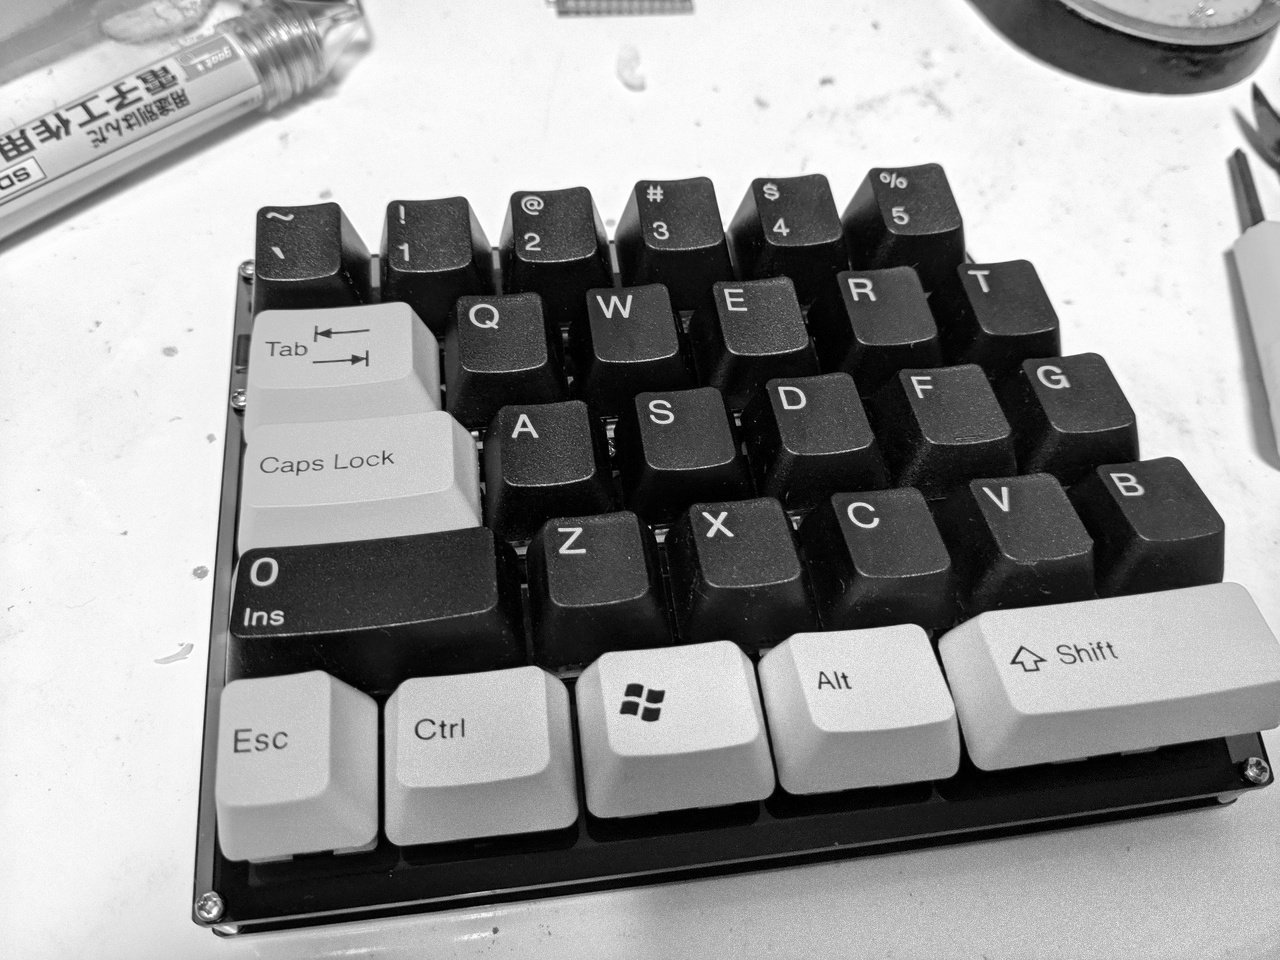
\includegraphics[keepaspectratio,width=5cm]{./image201911-kansai-02/mint60.jpg}
 \end{center}
 \vspace*{-1zw}
 \caption{Mint60 完成品(左半分)}
 \label{fig:mint60-katsu}
\end{figure}

\subsection{ファームウェアのカスタマイズ}

物理的にキーボードを作ったとしても、その後キーの配列を
自分の好みに合わていくという終わりの無い旅がはじまっていきます。
配列をいじるにはマイコンのファームを変更していくことになります。
キーボードのファームウェアについて、大体のキットが、qmk\_firmware%
\footnote{\url{https://github.com/qmk/qmk_firmware}}
という、ファームを焼くところまでmakeコマンド一発でできてしまう環境を使っています。

さて、ここでようやくDebianの影が見えますが、
このqmk\_firmwareを使用するためには、Debianの場合は以下のパッケージの
インストールが必要です。

\begin{commandline}
% sudo apt-get install gcc unzip wget zip gcc-avr binutils-avr avr-libc dfu-programmer dfu-util \
> gcc-arm-none-eabi binutils-arm-none-eabi libnewlib-arm-none-eabi
\end{commandline}

この状態で、まずはキーボードのキー配列を換えてみます。
といっても、実に簡単でして、
環境の \verb|keyboards/(キーボード名)/keymaps/(キーマップ名)/keymap.c|
を覗いてみると、以下のようなコードが記述されています。

\begin{commandline}
[0] = LAYOUT( \
KC_GRV,  KC_1,  KC_2,  KC_3,  KC_4,  KC_5,     KC_6,  KC_7,  KC_8,  KC_9,  KC_0,  KC_MINS, KC_EQL,   KC_BSPC,  \
KC_TAB,   KC_Q,  KC_W,  KC_E,  KC_R,  KC_T,     KC_Y,  KC_U,  KC_I,  KC_O,  KC_P,  KC_LBRC, KC_RBRC, KC_BSLS,  \
KC_CAPS,   KC_A,  KC_S,  KC_D,  KC_F,  KC_G,     KC_H,  KC_J,  KC_K,  KC_L,  KC_SCLN,KC_QUOT,        KC_ENT,   \
KC_LSFT,    KC_Z,  KC_X,  KC_C,  KC_V,  KC_B,     KC_N,  KC_M,  KC_COMM,KC_DOT,KC_SLSH,KC_RSFT,KC_UP,  MO(1),  \
KC_ESC,  KC_LCTL,KC_LGUI,KC_LALT,  MO(1),    KC_SPC, KC_ENT,  LALT(KC_GRV),           KC_LEFT,KC_DOWN,KC_RGHT  \
),
\end{commandline}

ええ、もうおわかりですね、上記の配列%
\footnote{\texttt{LAYOUT}がマクロ関数になってるので、配列に見えないかもしれませんが。}
を良い感じに書き換えるだけです。
Debianさわってるような人であれば、テキストファイルをさわるなんてなんの抵抗もないのではないでしょうか。

さて、よく見ると上記の配列にはファンクションキーの定義がありません。
もちろんそれらはキーの組み合わせで打つことになります。
上記の配列の場合、 \verb|MO(1)| となっているキーがありますが、
これを押しながら他のキーを押すと、上記の配列以外のキー入力としてPC側に送信できます。
なお、それらのコードも以下のような配列を変更するだけです。

\begin{commandline}
[1] = LAYOUT( \
KC_ESC, KC_F1, KC_F2,  KC_F3,  KC_F4,  KC_F5,    KC_F6,  KC_F7,  KC_F8,  KC_F9,  KC_F10, KC_F11, KC_F12,  KC_DEL, \
RGB_TOG, RGBRST,RGB_HUI,RGB_SAI,RGB_VAI,XXXXXXX,  XXXXXXX,XXXXXXX,XXXXXXX,XXXXXXX,XXXXXXX,XXXXXXX,XXXXXXX,XXXXXXX,\
XXXXXXX,  RGB_MOD,RGB_HUD,RGB_SAD,RGB_VAD,XXXXXXX, XXXXXXX,XXXXXXX,XXXXXXX,XXXXXXX,XXXXXXX,XXXXXXX,      XXXXXXX, \
_______,   XXXXXXX,XXXXXXX,XXXXXXX,XXXXXXX,XXXXXXX, XXXXXXX,XXXXXXX,XXXXXXX,XXXXXXX,XXXXXXX,_______,KC_PGUP,_______,\
XXXXXXX, _______,_______,_______,XXXXXXX,    XXXXXXX, XXXXXXX,XXXXXXX,                     KC_HOME, KC_PGDN, KC_END \
)
\end{commandline}

この後、以下のコマンドを叩き、キーボードのリセットスイッチを押せば
ファームウェアの更新が実行されます。

\begin{commandline}
% make (キーボード名):(キーマップ名):avrdude
\end{commandline}

また、このレイヤーの切り替えも、キーを押しながらだけでなく、
カナキーよろしくトグル動作といった具合にもできます。
その場合、現在のモードは、qmk\_firmwareに用意された仕組みでOLEDに表示させること等ができます。
これによって、QWERTYとDovrokを切り替えてつかったりもできるわけです。

もちろん、単純なキーではなく、ショートカットやら文字列入力を1キーに割り合てることもできます。
たとえば、Twitter廃人らしく、
``\verb|#debian #kansaidebian|'' を1キーで入力できるようにしてみます。
先程のキー配列のあったファイルに以下のようなenum値やマクロを追加し、

\begin{commandline}
enum macro_keycodes {
  KC_SAMPLEMACRO,
  KC_HASH_DEBIAN,  /* 追加 */
};

//Macros
#define M_SAMPLE M(KC_SAMPLEMACRO)
#define M_HASH_DEB M(KC_HASH_DEBIAN)  /* 追加 */
\end{commandline}

さらに配列を書き換え……、

\begin{commandline}
const uint16_t PROGMEM keymaps[][MATRIX_ROWS][MATRIX_COLS] = {

      /* 中略 */
      KC_HASH_DEBIAN,  KC_LCTL,KC_LGUI,KC_LALT,  MO(1),    KC_SPC, KC_ENT,  LALT(KC_GRV),     KC_LEFT,KC_DOWN,KC_RGHT  \
      /* 後略 */
\end{commandline}

最後に、キー入力の関数にcase文を追加すると……

\begin{commandline}
bool process_record_user(uint16_t keycode, keyrecord_t *record) {
  switch (keycode) {

    /* 中略 */

    case KC_HASH_DEBIAN:
      if (record->event.pressed)
        SEND_STRING("#debian #kansaidebian");
      break;

   /* 後略 */
\end{commandline}

1ボタンでdebian向けハッシュタグを打ててしまいます。
この機能を使うと、他にも例えばキーを短押ししたときは普通のキーとして、
長押ししたらレイヤー切り替えのキーとして動作する、といったような事もできます。
他にも、LEDはOLEDの制御等も色々と触れますが、
ProMicroだとファームサイズはそこまで大きくできませんので、ご注意ください。

\subsection{それでも満足できないアナタへ}

ここまで読んでいただいてわかるように、本当に自分のEndgameを目指すのであれば、
結局それに合ったキットがなければどうしようもありません。
ところで、最近はプリント基板ことPCBは気軽に作れるようになってきている……らしいです。
実際、10cmx10cmであれば、送料を考えなければ(ぉ) 5\$とかで作れてしまうようです。
ということで、Endgameのために基板から自作しましょう(錯乱)。
私もまだ志半ばですので、是非みなさんもご一緒に!!

基板設計ってどうやるの、と不安になるかもしれません。
しかしそこはご安心ください、PCBの設計用のツールはフリーのKiCadと呼ばれるソフトがあり、
ちゃんとDebianパッケージもございます(申し訳程度のDebian要素その2)。

\begin{commandline}
% apt search '^kicad$'
ソート中... 完了
全文検索... 完了
kicad/unstable,now 5.1.5+dfsg1-1 amd64 [インストール済み]
  電子回路および PCB 設計ソフトウェア
% apt install kicad
\end{commandline}

KiCadを入れたら、まずは回路図から作っています。
その際、キーボード用のパーツ(キースイッチとかProMicro)のライブラリが必要になりますが、
文献\cite{foostan01}にて、著者の方がKiCad用のライブラリを公開してくれています%
\footnote{\url{https://github.com/foostan/kbd}}。
この文献、この記事なんかよりも詳細なKiCadでの設計方法が書かれておりますので、
興味があれば是非お買い求めください。
ライブラリを適当な場所にcloneしたら、メニューの「シンボルライブラリーを管理」から登録できます。
例として、図\ref{fig:kicad-schematic}に、私がテストでつくりかけている4x4のキーボードの回路図を掲載しておきます。
左上にProMicroが、右上にキーマトリックス回路が見えてると思います。

\begin{figure}[htbp]
 \begin{center}
  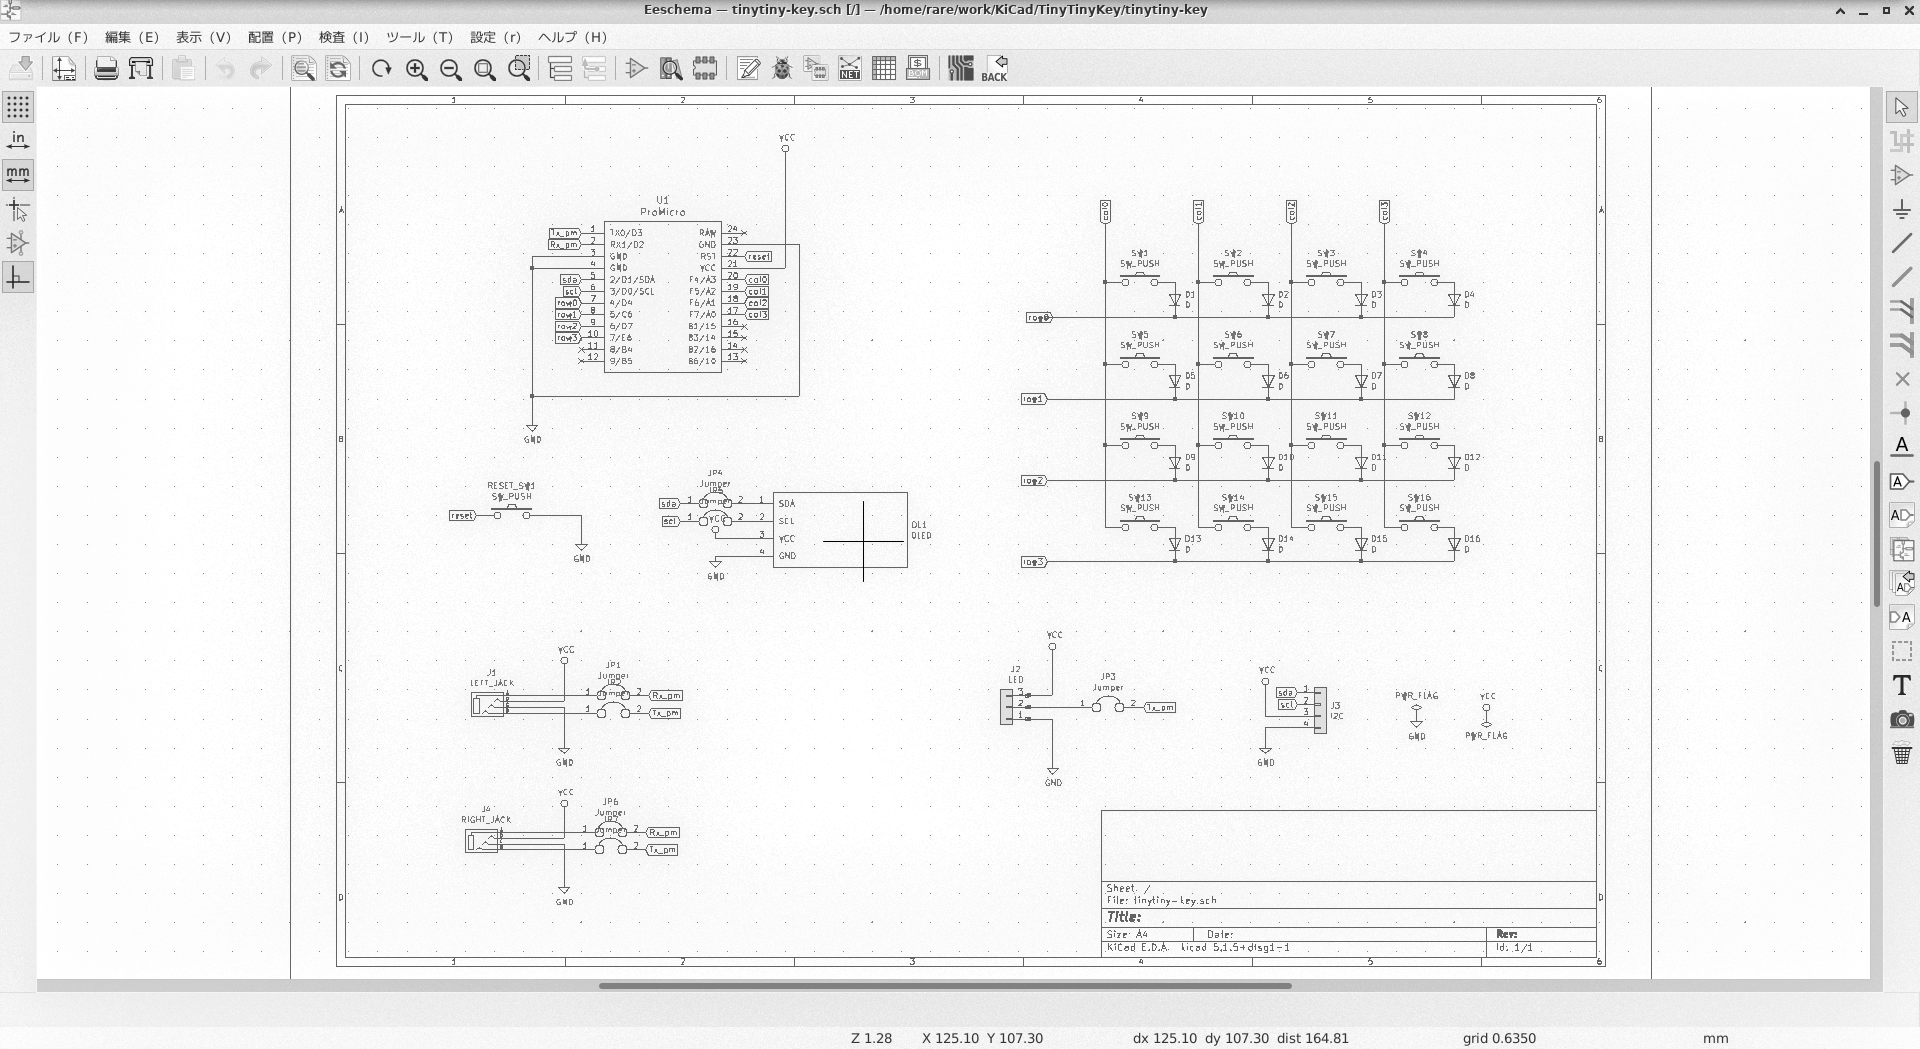
\includegraphics[keepaspectratio,height=5cm]{./image201911-kansai-02/kicad-schematic.png}
 \end{center}
 \vspace*{-1zw}
 \caption{KiCadの画面(回路図エディタ)}
 \label{fig:kicad-schematic}
\end{figure}

次に、フットプリント(基板上のはんだ付け部分)を回路と関連付けていくのですが、
その際にもフットプリントのライブラリが必要となります。
そちらのライブラリについても、\cite{foostan01}の著者の方が先程と同様の場所に公開してくれています。
作業としては、図\ref{fig:kicad-footprint}のような感じで、
回路図の各シンボルについて、どのフットプリントを適用するのかという事を
関連付けていくことになります。

\begin{figure}[htbp]
 \begin{center}
  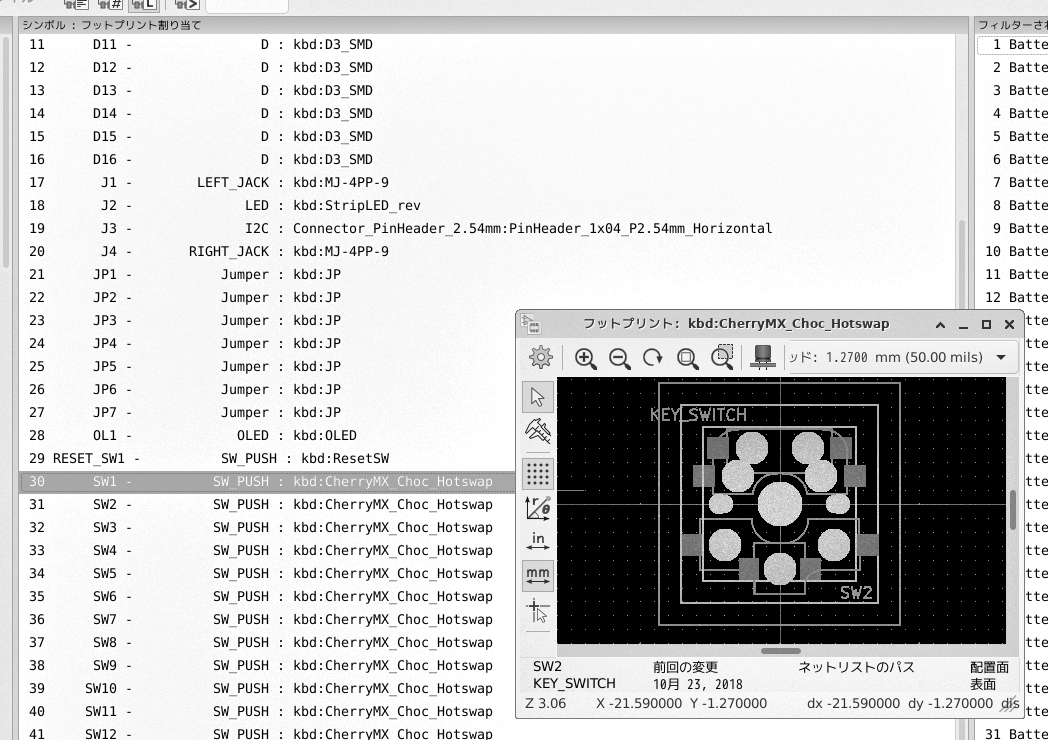
\includegraphics[keepaspectratio,height=5cm]{./image201911-kansai-02/kicad-footprint.png}
 \end{center}
 \vspace*{-1zw}
 \caption{KiCadの画面(フットプリントの関連付け)}
 \label{fig:kicad-footprint}
\end{figure}

フットプリントの関連付けが終わると、次はレイアウトになります。
パーツが干渉しないように注意して……やるのですが、
私はこの作業の途中で力尽きております……。
画面としては、図\ref{fig:kicad-footprint}のような感じになります。

\begin{figure}[htbp]
 \begin{center}
  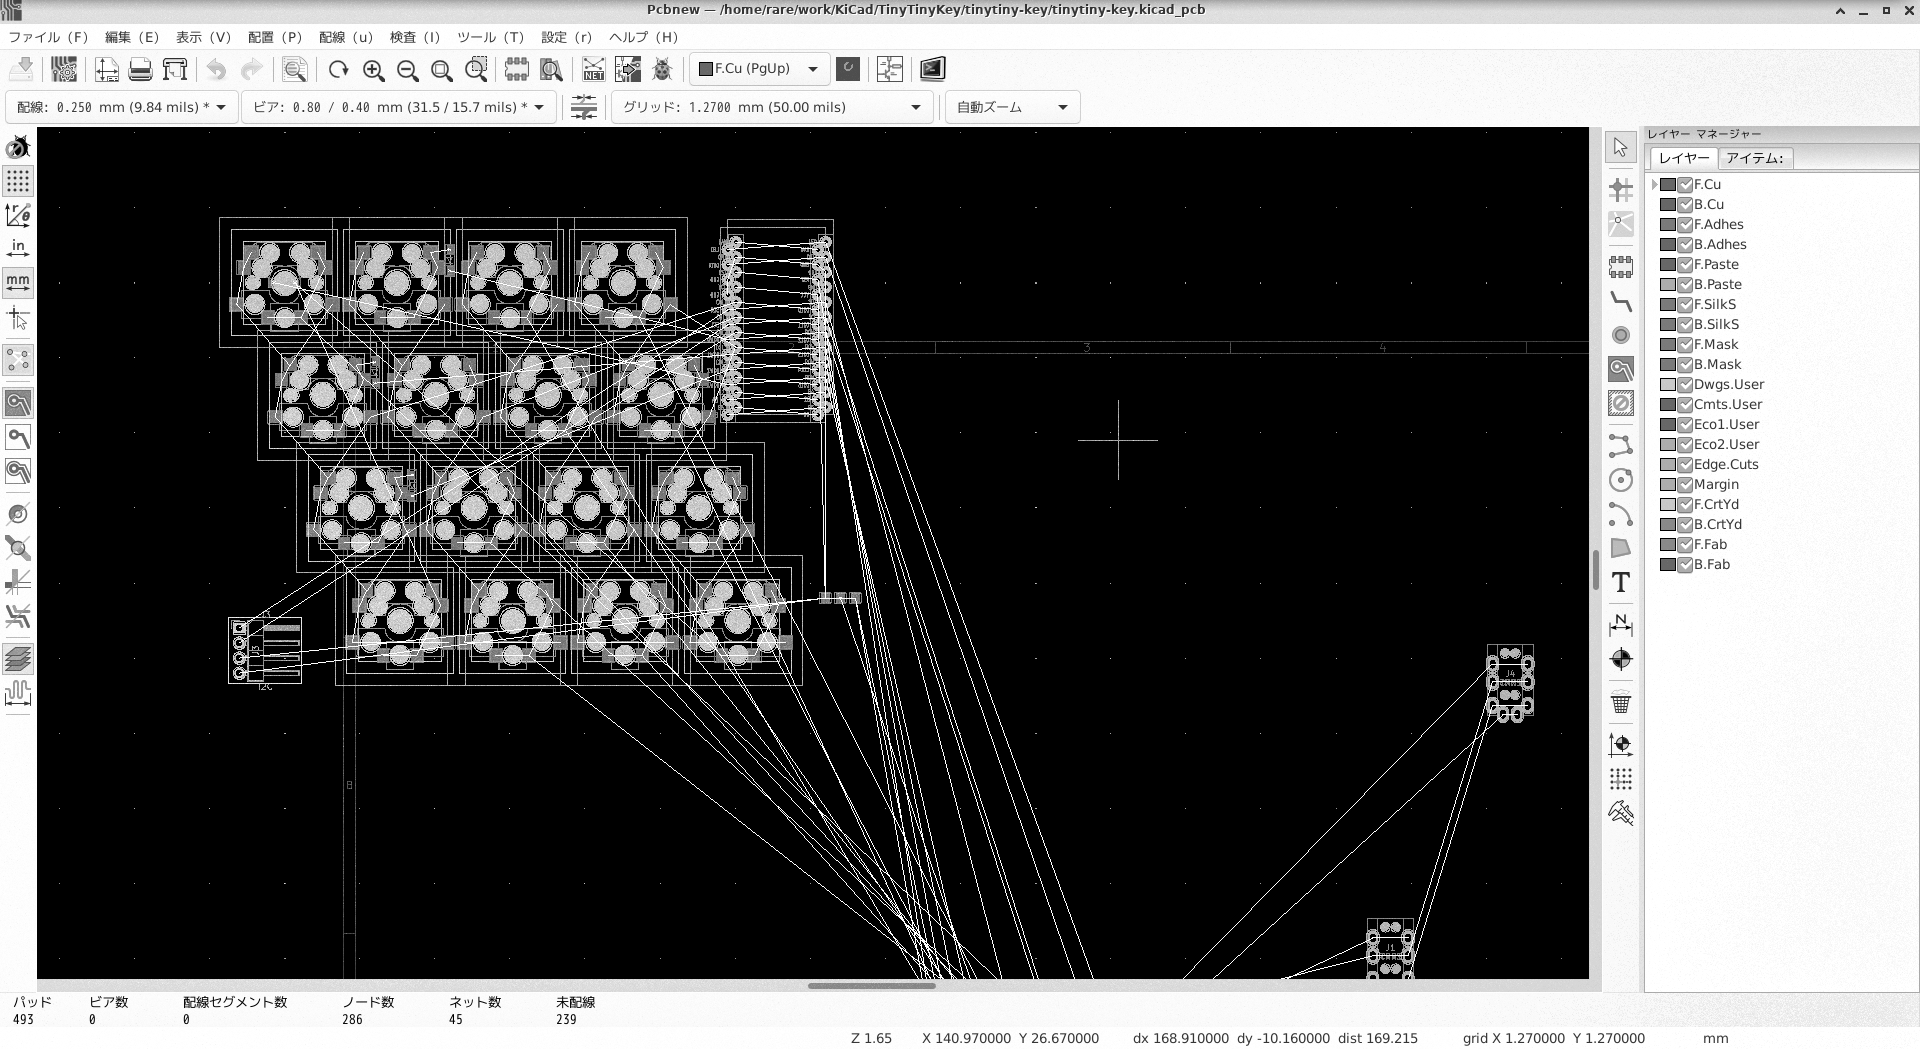
\includegraphics[keepaspectratio,height=5cm]{./image201911-kansai-02/kicad-layout.png}
 \end{center}
 \vspace*{-1zw}
 \caption{KiCadの画面(レイアウト……の途中で力尽きているところ)}
 \label{fig:kicad-footprint}
\end{figure}

その後の流れとしては、

\begin{enumerate}
 \item エッジカット線を引く
 \item スペーサー用の穴をあける
 \item 配線を実施する(一番大変らしい)
 \item 必要に応じてケースを作成する
       \begin{itemize}
	\item アクリル板を加工するのが主流
	\item 最近は3Dプリンタ勢が増えているみたい……
       \end{itemize}
\end{enumerate}

といったような感じになるようです。
PCB自体は、設計ができたらプリント基板の実装サービスをやっている場所に発注するようです。
seeed\footnote{\url{https://www.seeedstudio.com/fusion_pcb.html}}や
ELECROW\footnote{\url{https://www.elecrow.com/pcb-manufacturing.html}}
といったところがメジャーなようです。
海外なので送料はそこそこかかってしまいますが、
10cmx10cmのサイズであれば、相当安く作ってくれるようです。

なお、今回私は試しにと基板をまっサラなところから作成していますが、
実は回路図データを公開しているキットは結構あります。
先程紹介したHelixがその一つで、回路図がGitHub上に公開されています%
\footnote{\url{https://github.com/MakotoKurauchi/helix}}。
そのため、このHelixのPCBをベースにして作成されたキットも数多くあります。
なお、KiCadについては、文献\cite{foostan01}, \cite{kicad}あたりが参考になるかと思います。

\subsection{まとめ}

ということで、最後の基板からの自作については少々尻すぼみな感じになってしまいましたが、
キットから作るという選択肢を取れば、結構簡単に自作できてしまうのでした。
私は、分割式のキーボードを使うようになって、はや2ヶ月とか経ちますが、
腰痛に関しては冗談抜きで本当に改善しました。
以前は、一時間も座っていたら座っていられないくらい辛くなっていた腰痛が、
もちろんまったく痛くならないわけではないですが、座っていられないような事はなくなりました。
逆に、Fitbitに課される「1時間250歩」が全然クリアできなくなって困っております。

Debian勉強会で、この内容についてしゃべったところ、
自己紹介でのキーボード遍歴で大変に盛り上がりました。
おそらく、今回Debian本を読まれている方につきましても、
キーボードに関しては色々と語ることもあるかと思います。
\textbf{Debianをハックするには、まずは健康から!!どうでしょう、自作キーボード!!}
自作キーボードについては、「Self-Made Keyboards in Japan」というDiscordのサーバー\cite{discord}
に結構な情報が集まっています。
また、Discordはちょっと……という方には、Youtubeなどで情報を集めるのも良いかと思います。
「ほぼ週刊キーボードニュース」\cite{weekly}あたりはおすすめです。
本記事が、みなさまの健康的なハックライフに繋がると幸いです。

\subsection{参考文献}

\renewcommand{\refname}{\vspace*{-1.5zw}}
\begin{thebibliography}{9}
 \bibitem{foostan01} foostan, ``自作キーボード設計入門 Endgameへの第一歩'', \url{https://booth.pm/ja/items/1044084}
 \bibitem{kicad} 小坂貴美男, ``KiCad 5.0 / 5.1 入門実習テキスト『KiCad Basics for 5.x』``,
	 \url{https://booth.pm/ja/items/941963}
 \bibitem{discord} \texttt{@Biacco42}, ``Self-Made Keyboards in Japan'', \url{https://discordapp.com/invite/NM7XtDW}
 \bibitem{weekly} \texttt{@Biacco42} and \texttt{@Pekaso},``ほぼ週刊キーボードニュース'', \url{https://www.youtube.com/channel/UCyU1PAGvw_suAyI4wljHmag}
\end{thebibliography}

%-------------------------------------------------------------------------------
\dancersection{Debian GNU/kFreeBSD セットアップガイド 2019年版}{杉本典充}
%-------------------------------------------------------------------------------

\subsection{はじめに}

Debian Project では Debian GNU/Linux という Linux ディストリビューションを開発しており多くの開発者及び利用者がいます。Debian Project では ユニバーサルなオペレーティングシステムを提供する考え方をもっており、その理念に則り FreeBSD カーネルで動作する Debian GNU/kFreeBSD という別の OS\footnote{Linux カーネルでなく FreeBSD カーネルでもない Debian GNU/Hurd というものもあります。} があります。

Debian GNU/kFreeBSD はその特異さゆえに Debian GNU/Linux と異なる点が多くあります。今記事では Debian GNU/kFreeBSD を触れるにあたり、どのようにセットアップを行うとよいか説明します。


\subsection{Debian Ports と Debian GNU/kFreeBSD}

\subsubsection{Debian Ports とは}

Debian Ports\footnote{\url{https://www.ports.debian.org/}}とは、さまざまなCPUやカーネルで動作するように移植を行うプロジェクトです。

FreeBSD カーネルで動作する Debian を作るプロジェクトがあり、その Debian のことを「Debian GNU/kFreeBSD」と呼んでいます ("k" は kernel のこと)。現在ではIntel CPUのアーキテクチャのみあります (kfreebsd-amd64、kfreebsd-i386)。

\subsubsection{Debian GNU/kFreeBSD のリリースの歴史}

Debian GNU/kFreeBSD のリリースの歴史は以下となっています。

\begin{itemize}
\item 2011年2月6日、Debian 6 (squeeze) おいてテクノロジープレビューとして stable 版をリリース。ftp.debian.org にてパッケージの配布を開始。
\item 2013年5月4日、Debian 7 (wheezy) において stable 版をリリース。
\item 2014年9月、Debian 8 (jessie) でリリースするアーキテクチャを選定する過程で、kFreeBSD は開発や保守に関わる人が少なく stable の維持と新規開発の両立ができていない状況が見られることを指摘される\footnote{\url{https://lists.debian.org/debian-devel-announce/2014/09/msg00002.html}}。その指摘を改善できなかったため、Debian 8 (jessie)では stable 版のリリースは見送られる\footnote{過去バージョンの利用者が困るであろうということで jessie-kfreebsd 版という裏バージョンが存在していた。}。
\item Debian 9 (stretch) においても stable 版のリリースはされない状況が続く\footnote{stretch-kfreebsd 版はリリースされませんでした。}。
\item 2018年5月31日、Debian 7 (wheezy) の LTS が終了。これにて Debian GNU/kFreeBSD の stable 版はサポートを終了。
\item Debian 10 (buster) のリリースに向けて ftp.debian.org の整理を実施。
\item 2019年5月25日、Debian GNU/kFreeBSD は Debian Ports(\url{https://www.ports.debian.org/}) へ移転。これにより ftp.debian.org におけるパッケージの配布を終了。
\end{itemize}

\subsubsection{Porterbox}

Debian Project では多くのアーキテクチャを開発しているため、移植作業用にサーバを借りる「porterbox」という仕組みがあります\footnote{\url{https://wiki.debian.org/PorterBoxHowToUse}}\footnote{実際に借りた事例の報告「Debianの移植作業用のインフラを借りるには」\url{https://tokyodebian-team.pages.debian.net/pdf2016/debianmeetingresume201603.pdf}}。

bugreportにはあるアーキテクチャのみで発生する不具合も報告されますが、パッケージをメンテナンスしている人がそのアーキテクチャの環境を持っていない場合があります。その場合は環境を自分で構築するか、porterboxを利用してバグの修正作業を行います。

なお、Debian GNU/kFreeBSD では kfreebsd-amd64 の porterbox "lemon.debian.net" を運用しています\footnote{\url{https://db.debian.org/machines.cgi?host=lemon}}\footnote{"New GNU/kFreeBSD Porterbox" \url{https://lists.debian.org/debian-devel/2019/02/msg00313.html}}。


\subsubsection{Debian GNU/kFreeBSD 固有の Debian パッケージ}

Debian GNU/kFreeBSD固有のパッケージの例を紹介します。

\subsubsubsection{kfreebsd-imageパッケージ}

Debian GNU/kFreeBSD の kernelイメージを収録したパッケージです。Debian Ports の kFreeBSD では kfreebsd-image-10.3 が利用できます。experimental には kfreebsd-image-11 があります\footnote{FreeBSD の最新版は 2018年12月11日にリリースした FreeBSD-12.0です。}。

\subsubsubsection{zfsutilsパッケージ}

zfsutils パッケージは ZFS を操作するコマンドを含んだパッケージです。インストール時のファイルシステムに ZFS を選択した場合はデフォルトでインストールされます。

%kfreebsd-image-10.3 で利用できるZFSのバージョンは ver NN となっています。
%
%\begin{commandline}
%  $ zpool upgrade -v
%  (snip)
%  NN  Multiple vdev replacements
%\end{commandline}

\subsubsubsection{freebsd-utilsパッケージ}

freebsd-utilsパッケージは、FreeBSD固有のコマンドを含んだパッケージです。/sbin/mount\_*、/usr/sbin/jailなどが入っています。

\subsubsubsection{freebsd-net-toolsパッケージ}

freebsd-net-toolsパッケージは、FreeBSD向けのネットワーク操作のコマンドを含んだパッケージです。arp、ifconfig、netstat、routeコマンドなどが入っています。

\subsubsubsection{freebsd-smbfsパッケージ}

freebsd-smbfs パッケージは、Windows ファイル共有(SMB共有)へアクセスするためのパッケージです。
インストールすると、"/usr/sbin/mount\_smbfs" コマンドが使えるようになります。

Windows ファイル共有先を mount するには以下のコマンドを実行します。

\begin{commandline}
# mount_smbfs -E UTF-8:CP932 -I {ファイルサーバのIPアドレス} -U {smbユーザ名} //{ファイルサーバのIPアドレス}/{dir} {mount先dir}
\end{commandline}

\subsubsubsection{freebsd-pppパッケージ}

freebsd-pppパッケージは、ダイアルアップする "/usr/sbin/ppp" コマンドを含んでいます。3G や LTE に対応した USB モデムを使う場合に必要となります。

Debian GNU/Linux では ppp パッケージや wvdial パッケージでダイアルアップしますが、kfreebsd ではそれらは使えないため注意が必要です。

\subsubsubsection{pfパッケージ}

FreeBSD kernelがもつ Packet Filter と呼ばれるいわゆるファイアウォール機能を制御するコマンド "/sbin/pfctl" を含んだパッケージです。

/sbin/pfctl の設定ファイルは "/etc/pf.conf" であり、Linuxのiptables用設定ファイルと中身が全く異なります。


\subsection{Debian GNU/kFreeBSDのインストール}

\subsubsection{インストールするPC}

今回は ThinkPad X220 という Intel の Sandy Bridge 世代のノートPCにインストールをしてみます。このノートPCの有線LANと無線LANのチップは Intel 製であり FreeBSD カーネルの標準でドライバが提供されているため認識させやすいです。


\subsubsection{インストールイメージの入手}

開発者向けの Debian Installer は通常 \url{https://www.debian.org/devel/debian-installer/} で配布しています。しかし、Debian GNU/kFreeBSD は Debian Ports へ移行したため、\url{https://www.debian.org/devel/debian-installer/} にある kFreeBSD 用インストーラは動作しなくなっています。

代わりに非公式版の Debian Installer の ISO イメージが用意されており、以下の ISO ファイルを利用してインストールします。

通常は kfreebsd-amd64 版\footnote{\url{http://jenkins.kfreebsd.eu/jenkins/view/cd/job/debian-cd_sid_kfreebsd-amd64/ws/build/debian-unofficial-kfreebsd-amd64-NETINST-1.iso}}を使うとよいでしょう。
kfreebsd-i386 版\footnote{\url{http://jenkins.kfreebsd.eu/jenkins/view/cd/job/debian-cd_sid_kfreebsd-i386/ws/build/debian-unofficial-kfreebsd-i386-NETINST-1.iso}}を利用しても構わないのですが、ファイルシステムに ZFS を使う場合はメモリ不足になりがちなため注意してください。

ISO ファイルをCD/DVD メディアへ焼いてインストールディスクを作成し、インストールディスクから PC を起動すると Debian Installer が起動します。


\subsubsection{インストーラの表示言語}

kfreebsd 版 Debian Installerは、日本語の表示ができません(インストーラでフレームバッファが有効になっていないと思われる)。そのため、LANG=Cでインストールを進めます。


\subsubsection{パーティション構成とファイルシステム}

Debian GNU/kFreeBSD を MBR 方式でブートする環境へインストールする場合は root パーティションを MBR の基本パーティションにする必要があります\footnote{もし Debian GNU/Linux や Windows とデュアルブートしたい場合は、MBR方式では基本パーティションの作成は4つまでという制約を考慮したパーティション構成にする必要があります。}(拡張パーティションにインストールすると grub のインストールに失敗します)。kFreeBSDを占有する環境の場合は以下のパーティション構成でよいでしょう(以下では "/dev/ada0p1" のファイルシステムに UFS を選択しています)。

\begin{commandline}
# fdisk -l /dev/ada0

Disk /dev/ada0: 238.5 GiB, 256060514304 bytes, 500118192 sectors
Units: sectors of 1 * 512 = 512 bytes
Sector size (logical/physical): 512 bytes / 512 bytes
I/O size (minimum/optimal): 512 bytes / 512 bytes
Disklabel type: dos
Disk identifier: 0x88f37f78

Device      Boot     Start       End   Sectors   Size Id Type
/dev/ada0p1           2048 273436671 273434624 130.4G a5 FreeBSD
/dev/ada0p2      273436672 281249791   7813120   3.7G 82 Linux swap / Solari
\end{commandline}

ファイルシステムは通常の利用する分には UFS を選択することが多いです。他には ZFS というスナップショット機能をもち多数のストレージを扱えるファイルシステムを選択することができます。


\subsubsection{パッケージをダウンロードするミラーサーバの指定}

Debian Installer が利用するミラーサーバは \url{http://deb.debian.org/debian/} がデフォルトになっています。しかし、kfreebsd-amd64 のパッケージは ftp.ports.debian.org にて配布しているためデフォルト値は利用できません。ひとまずミラーは利用しない選択をして処理を進めて "Standard system utilities" のみをインストールします\footnote{\url{http://ftp.ports.debian.org/debian-ports/} を指定すればよさそうなものなのですが、入力してもパッケージが見つからないエラーが起こり、先に進めませんでした。}。


\subsection{Debian GNU/kFreeBSDのセットアップ}

\subsubsection{有線LAN}

有線LANは利用するドライバによってデバイス名が変化します(IntelのPC向けの場合は"em0"、realtekの場合は"re0")。

設定ファイルは Debian GNU/Linux と同じ "/etc/network/interfaces" を参照しますが、allow-hotplug 句はlinuxで使われるudevが提供している機能であることから kfreebsd では利用できず注意が必要です。

そのため、有線LAN接続環境がない状況でOSを起動すると有線LANによるDHCPのIPアドレス取得がタイムアウトするまでloginプロンプトが出てこなくなります(起動に時間がかかる)。私はノートPC に Debian GNU/kFreeBSD をインストールする場合は以下コマンドを手動で実行してネットワークへ接続するようにしています。

\begin{commandline}
# vi /etc/network/interfaces

#auto em0  <-コメントにします
iface lan_home inet dhcp
\end{commandline}

\begin{commandline}
# ifup em0=lan_home
\end{commandline}

なお、ネットワークインタフェースの状態確認は昔ながらの"ifconfig"コマンドを利用してください(最近の linux と違い ip コマンドはありません)。

\subsubsection{aptの設定}

インストール時にミラーを指定しなかったため、/etc/apt/sources.list ファイルは中身がない状態になっています。

/etc/apt/sources.list は以下を設定します\footnote{\url{https://lists.debian.org/debian-bsd/2019/08/msg00005.html}}。

\begin{commandline}
# vi /etc/apt/sources.list
  
deb-src http://ftp.se.debian.org/debian/ sid main contrib non-free
deb http://ftp.ports.debian.org/debian-ports sid main
deb http://ftp.ports.debian.org/debian-ports unreleased main
deb-src http://ftp.ports.debian.org/debian-ports unreleased main
deb http://ftp.ports.debian.org/debian-ports experimental main
\end{commandline}

上記の apt の設定を行い apt-get コマンドを実行すると、 GPG キーエラーが発生して先に進めません。手動で keyring をインストールします。

\begin{commandline}
# wget http://ftp.jp.debian.org/debian/pool/main/d/debian-ports-archive-keyring/debian-ports-archive-keyring_2018.12.27_all.deb
# dpkg -i debian-ports-archive-keyring_2018.12.27_all.deb
\end{commandline}

これで apt-get が動作するようになります。他の keyring も更新しておきましょう。

\begin{commandline}
# apt-get update  
# apt-get install debian-keyring debian-archive-keyring
\end{commandline}


\subsubsection{localeの設定}

Debian Installerでは LANG=C を選択してインストールしているため、出力メッセージが英語になっています。そのためlocaleを日本語に変更します(ただし、コンソール環境では日本語メッセージが化けるため C.UTF-8 の方がデバッグしやすいかもしれません)。

\begin{commandline}
# dpkg-reconfigure locales

  -> ja_JP.UTF-8を選択する
\end{commandline}


\subsubsection{sshdのインストール}

openssh-serverパッケージを利用できます。以下コマンドでインストールできます。

\begin{commandline}
# apt-get install openssh-server
\end{commandline}


\subsubsection{無線LAN}

\subsubsubsection{無線LANのハードウェアの設定}

ThinkPad X220に搭載している無線LANチップは「Intel Centrino advanced-N 6205」です。

無線LANを利用するためにまずはメーカーが配布する無線LAN用firmwareをインストールします。
ただ、/etc/apt/sources.list に non-free のバイナリパッケージのダウンロード先を指定をしていないため、パッケージを直接ダウンロードしてインストールします。reboot して firmware を認識すると、dmesg に出力されていたファームウェアがロードできないというエラーがなくなります。

\begin{commandline}
# wget http://ftp.se.debian.org/debian/pool/non-free/f/firmware-nonfree/firmware-iwlwifi_20190717-2_all.deb
# dpkg -i firmware-iwlwifi_20190717-2_all.deb
# reboot
\end{commandline}

無線LANの通信を制御するデーモンである wpasupplicant パッケージ をインストールします。

\begin{commandline}
# apt-get install wpasupplicant
# wpa_supplicant -v
wpa_supplicant v2.4
Copyright (c) 2003-2015, Jouni Malinen <j@w1.fi> and contributors
\end{commandline}


\subsubsubsection{無線LANのネットワーク設定}

FreeBSD は物理無線LANインタフェースと論理無線LANインタフェースに分かれています。

ThinkPad X220に搭載しているIntel製無線LANチップの場合は "iwn0" という物理無線LANインタフェースがあります。

\begin{commandline}
# ifconfig iwn0

iwn0: flags=8802<BROADCAST,SIMPLEX,MULTICAST> metric 0 mtu 2290
        ether yy:yy:yy:yy:yy:yy
        media: IEEE 802.11 Wireless Ethernet autoselect (autoselect)
        status: no carrier
        nd6 options=23<PERFORMNUD,ACCEPT_RTADV,AUTO_LINKLOCAL>
\end{commandline}

以下のコマンドで論理無線LANインタフェースを生成します。"wlan0"というインタフェースが生成されました。

\begin{commandline}
# ifconfig wlan create wlandev iwn0
wlan: Ethernet address: yy:yy:yy:yy:yy:yy
wlan0

# ifconfig wlan0
wlan0: flags=8802<BROADCAST,SIMPLEX,MULTICAST> metric 0 mtu 1500
        ether yy:yy:yy:yy:yy:yy
        ssid " channel 1 (2412 MHz 11b)
        country US authmode OPEN privacy OFF txpower 14 bmiss 10 scanvalid 60
        bgscan bgscanintvl 300 bgscanidle 250 roam:rssi 7 roam:rate 1 wme
        bintval 0
        media: IEEE 802.11 Wireless Ethernet autoselect (autoselect)
        status: no carrier
        nd6 options=23<PERFORMNUD,ACCEPT_RTADV,AUTO_LINKLOCAL>
\end{commandline}

接続する無線LANアクセスポイントの認証情報設定ファイルを作成します。

\begin{commandline}
$ wpa_passphrase apname1 appassword > wpa_apname1.conf
$ cat wpa_apname1.conf
network={
        ssid=''apname1''
        #psk=''appassword''
        psk=e9fdcb43eba09b6342df30f14275625c8494e534799a82d6639b6124434ea627
}
\end{commandline}

無線LANアクセスポイントへ接続し、DHCPでIPアドレスを取得します。IPアドレスは論理インタフェースに付与されます。

\begin{commandline}
# wpa_supplicant -i wlan0 -c ./wpa_apname1.conf
Successfully initialized wpa_supplicant
ioctl[SIOCS80211, op=20, val=0, arg_len=7]: Invalid argument
ioctl[SIOCS80211, op=20, val=0, arg_len=7]: Invalid argument
wlan0: Trying to associate with zz:zz:zz:zz:zz:zz (SSID='apname1' freq=2427 MHz)
wlan0: Associated with zz:zz:zz:zz:zz:zz
wlan0: WPA: Key negotiation completed with zz:zz:zz:zz:zz:zz [PTK=CCMP GTK=CCMP]
wlan0: CTRL-EVENT-CONNECTED - Connection to zz:zz:zz:zz:zz:zz completed [id=0 id_str=]
wlan0: WPA: Group rekeying completed with zz:zz:zz:zz:zz:zz [GTK=CCMP]
\end{commandline}

\begin{commandline}
# dhclient wlan0

# /sbin/ifconfig wlan0
wlan0: flags=8843<UP,BROADCAST,RUNNING,SIMPLEX,MULTICAST> metric 0 mtu 1500
        ether yy:yy:yy:yy:yy:yy
        inet6 fe80::a288:b4ff:fe18:b514%wlan0 prefixlen 64 scopeid 0x6
        inet 192.168.1.5 netmask 0xffffff00 broadcast 192.168.1.255
        ssid apname1 channel 4 (2427 MHz 11g) bssid zz:zz:zz:zz:zz:zz
        country US authmode WPA2/802.11i privacy ON deftxkey UNDEF
        AES-CCM 3:128-bit txpower 15 bmiss 10 scanvalid 60 bgscan
        bgscanintvl 300 bgscanidle 250 roam:rssi 7 roam:rate 5 protmode CTS
        wme roaming MANUAL
        media: IEEE 802.11 Wireless Ethernet OFDM/54Mbps mode 11g
        status: associated
        nd6 options=23<PERFORMNUD,ACCEPT_RTADV,AUTO_LINKLOCAL>
\end{commandline}


\subsubsubsection{無線LAN接続のトラブル}

wpa\_supplicantコマンドで無線LANアクセスポイントへ接続を試みたがエラーが発生し接続できない場合があります。その場合は以下を試すと接続できる場合があります。

\begin{itemize}
  \item 接続先SSIDを2.4GHz帯のものに変更する。
  \item "\# ifconfig wlan0 -ht40"を実行する。\footnote{デュアルチャネル接続を無効にして、20MHz幅の電波で通信するように指示するコマンドです。筆者の自宅で利用しているNEC製Wifiルータ Aterm に接続するにはこれを指定しないとうまくつながりませんでした。}
\end{itemize}


\subsubsection{音の再生}

FreeBSD は OSS (Open Sound System) という仕組みで音声出力をします(ALSA は Linux 専用のサウンドシステムです)。最近のPCには High Definition Audio 規格のチップが搭載されることが多いため、snd\_hda.ko ドライバでサウンドを出力することができます(snd\_hda.ko は FreeBSD kernel に static link されています)。

以下のコマンドを実行すると、コンソール上でMP3形式の音声ファイルを再生できます。

\begin{commandline}
# apt-get install mpg123
# mpg123 ${mp3ファイルのパス}
\end{commandline}
    

\subsubsection{電源関係}

CPUクロックの制御は powerd パッケージの powerd が行っています。現在動作中の CPU クロック数は sysctl コマンドで取得できます。

電源に接続時は 2501 MHz で動作しています。

\begin{commandline}
# sysctl dev.cpu.0.freq
dev.cpu.0.freq: 2501
\end{commandline}

電源に接続しておらずバッテリー動作時は 800 MHz で動作しています。

\begin{commandline}
# sysctl dev.cpu.0.freq
dev.cpu.0.freq: 800
\end{commandline}

バッテリー残量を取得するには acpiconf コマンドを実行します。

\begin{commandline}
# /usr/sbin/acpiconf -i 0

Design capacity:        57240 mWh
Last full capacity:     51530 mWh
Technology:             secondary (rechargeable)
Design voltage:         10800 mV
Capacity (warn):        2576 mWh
Capacity (low):         200 mWh
Low/warn granularity:   1 mWh
Warn/full granularity:  1 mWh
Model number:           45N1172
Serial number:            641
Type:                   LION
OEM info:               SANYO
State:                  high
Remaining capacity:     99%
Remaining time:         unknown
Present rate:           0 mW
Present voltage:        12154 mV
\end{commandline}

サスペンドとハイバーネートについては未確認です。


\subsubsection{KMSの有効化}

KMS(kernel mode settings)を有効にするとコンソール画面の解像度が上がります。i915.ko がKMS非対応で、i915kms.ko がKMS対応のカーネルモジュールです。これらのカーネルモジュールを利用するときはどちらかひとつのみロードします。

以下コマンドで KMS を有効にできます。

\begin{commandline}
# kldunload i915
# kldload i915kms
\end{commandline}

再起動後も自動でkernel moduleをロードするには以下のように設定します。

\begin{commandline}
# vi /etc/modules
i915kms
\end{commandline}


\subsubsection{X Window System}

\subsubsubsection{X Window System用ビデオドライバ}

ThinkPad X220はIntelのオンボードGPUを搭載しています。そのため、ビデオドライバは xserver-xorg-video-intel を利用します。インストーするには以下のコマンドを実行します。

\begin{commandline}
# apt-get install xserver-xorg-video-intel
\end{commandline}

今の kFreeBSD で安定動作させるには Intel のドライバの動作モードを古いUXAモードに変更するとよいようです。

\begin{commandline}
# vi /etc/X11/xorg.conf.d/50-intel.conf
Section ``Device''
  Identifier  ``Card0''
  Driver      ``intel''
  Option      ``AccelMethod''  ``uxa''
EndSection
\end{commandline}


\subsubsubsection{ウィンドウマネージャ}

twmをインストールすることが可能です。それ以外のicewm、xfce4、lxdeなどはパッケージの依存関係が解決できない状態のためインストールできません。グラフィカルログインマネージャのxdm、lightdmもパッケージの依存関係が解決できない状態のためインストールできません。

ターミナルエミュレーターも必要になるため、xterm、etermをインストールしておきます。

\begin{commandline}
# apt-get install twm xterm eterm
\end{commandline}

コンソール環境において root ユーザで startx コマンドを実行すると twm を起動できます。

\begin{commandline}
# startx
\end{commandline}

twmの画面上で左クリックをするとメニューが表示されますので、eterm を起動すればCLIの操作ができます\footnote{xterm は "open ttydev: No such file or directory" というエラーが出て起動できませんでした。}。


\subsection{Debianの開発ツールのセットアップ}

\subsubsection{インストールできるパッケージ}

以下のパッケージは、/etc/apt/sources.list に設定したリポジトリからバイナリパッケージをインストールできます。

\begin{itemize}
\item make / bmake
\item gcc-9 / g++-9
\item clang-7
\item dpkg-dev
\item devscripts
\item build-essential
\item debhelper
\item debootstrap
\item subversion
\item vim
\end{itemize}

\subsubsection{インストールができない状態になっているパッケージ}

以下のパッケージは ftp.ports.debian.org のあるパッケージ群で依存関係が壊れているためインストールできないパッケージです。

\begin{itemize}
\item clang-8
\item git
\item emacs / emacs-nox
\end{itemize}


\subsection{その他の機能の紹介}

\subsubsection{コンテナ環境:Jail}

FreeBSDにはFreeBSD Jailというコンテナ型仮想化環境を実行する機能があります。freebsd-utilsパッケージをインストールすることでコンテナを操作するコマンド群をインストールすることができます。コンテナ環境の作成は debootstrap、コンテナ環境の操作は jail、jls、jexec などが利用できます。

\begin{commandline}
# debootstrap --no-check-gpg sid ./jail_demo_1 http://ftp.ports.debian.org/debian-ports/
\end{commandline}

以下コマンドでchrootコマンドのようにjail環境に入れます\footnote{hostnameを指定するオプション、ipv4アドレスを指定するオプションは省略しています。}。

\begin{commandline}
# jail -c path=./jail_demo_1 command=/bin/bash
\end{commandline}

jail環境を起動した後は、jlsコマンドでjidを取得し、jexecでjail環境の中で任意のコマンドを実行できます。

\begin{commandline}
# jls
JID  IP Address      Hostname                      Path
  1  -                                             /root/jail/jail_1

# jexec 1 cat /etc/debian_version
\end{commandline}


\subsubsection{Linuxエミュレーション}

debootstrap で Debian 6 squeeze の linux-i386 の コンテナ環境を作成しようとしたところエラーが発生しました\footnote{kfreebsd-image-10.3 の linux.ko は linux-2.6.32 の 32bit ABI のエミュレーションだったと記憶しています。}。

現在は動かないのかもしれません。

\begin{commandline}
# debootstrap --no-check-gpg --arch=i386 squeeze ./linux_demo_1 http://archive.debian.org/debian/
ELF binary type "0" not known.
E: Unable to execute target architecture
\end{commandline}


\subsubsection{完全仮想化環境}

FreeBSD には OS を完全仮想化して動作させる virtualbox、bhyveがありますが、Debian GNU/kFreeBSDにはまだ移植されていません。


\subsection{おわりに}

Debian GNU/kFreeBSD のインストール方法とセットアップ方法について説明しました。bugreport で kfreebsd 環境で動かないと報告がある場合や kfreebsd を開発してみたい方は参考にしてみてください。

%-------------------------------------------------------------------------------
\dancersection{DebConf19 の気になるセミナーを調べてみる}{杉本典充}
%-------------------------------------------------------------------------------

\subsection{はじめに}

DebConf19 が 2019年7月21日から28日にブラジルのクリチバ市で開催されました。

\url{https://debconf19.debconf.org/}

多くのセミナー発表があり、現在のDebian Projectのトレンドをつかむことができます。このセミナーはビデオ公開しているセミナーも多いため、ビデオを見てみてどんな内容だったのか調べてみました。

\subsection{DebConf19のセミナービデオ}

\subsubsection{セミナースケジュールとビデオの場所}

DebConf19のセミナースケジュールは以下のURLで公開しています。

\url{https://debconf19.debconf.org/schedule/}

このURLのページ内にある各セミナーのタイトルをクリックするセミナーの概要のぺージが表示され、セミナーによってはスライドとビデオが見れるようになっています。


\subsubsection{気になるセミナー}

私が個人的に気になるセミナーは以下です。

\begin{itemize}
\item i'm (a bit) sick of maintaining piuparts.debian.org (mostly) alone, please help (20min)
\item APT 2.0 and other news (20min)
\item Using Debian Containers for Cross-Development (45min)
\item Debian LTS, the good, the bad and the better (45min)
\item Who's afraid of Spectre and Meltdown? (45min)
\item Escaping the Surveillance Blackhole with Free Mobile Computing (45min)
\item Bootstrappable Debian BoF (45min)
\item debian/copyright BoF (45 min)
\item Bits from the DPL (45min)
\end{itemize}


\subsection{ビデオを見てみたセミナー}

\subsubsection{APT 2.0 and other news}

%スライドデータ
%
%\url{https://salsa.debian.org/debconf-team/public/share/debconf19/raw/master/slides/79-apt-20-and-other-news.pdf?inline=false}

\begin{itemize}
\item  Ubuntu 14.04のESMが始まった
  \begin{itemize}
  \item public dist/、 private pool/ が要件。認証処理が必要
  \item ''never'' pin という仕組みを考えた  
  \end{itemize}
\item 2018年にfrontend lockを導入
  \begin{itemize}
  \item 主に python-apt が抱える不具合を修正
  \item Ubuntu errerトラッカーの情報では unattended-upgrades によるcrachの報告が減った
  \end{itemize}
\item アップデート中にシャットダウンした場合の問題への対応
  \begin{itemize}
  \item apt 1.8.1 以降では、systemdへshutdownしないように制御できるようになった
  \item systemctlやGUIツールの実行中はshutdownしないように防ぐことができる
  \item sudo rebootや似たようなコマンドはまだ対応していない
  \end{itemize}
\item busterへdist-upgradeするときにエラーが出たのは申し訳なかった
  \begin{itemize}
  \item エラー内容
    \begin{itemize}
    \item E: Repository ’foo’ changed its ’Suite’ value from ’testing’ to ’stable’
    \item E: Repository ’bar’ changed its ’Codename’ value from ’buster’ to ’bullseye’
   \end{itemize}
  \item 何がやりたかったのか
    \begin{itemize}
    \item Security: Prevent people from giving you stable when you ask for stable-security
    \item Pinning: Prevent broken pinning situations
     \end{itemize}
  \item どうすればよかったのかの案を考えてみたので、みなさんと議論してみたいです
  \end{itemize}
\item dpkgのnews
  \begin{itemize}
  \item Trigger loops might finally be over
  \item Rootless ビルドできるようになった
  \item start-stop-daemon は新しい systemd の readiness protocol に対応
  \item CPANにDpkg perlモジュールが入りました
  \item クロスコンパイルサポートの改善    
  \end{itemize}
\item APT 2.0
  \begin{itemize}
  \item できるかどうかわからないこと
    \begin{itemize}
    \item ``purge''、''installed''、''config-files'' などでパターンマッチング指定を採り入れたい
    \item pinningもパターンマッチング指定を採り入れたい
    \item Pin and upgrade by source package ?
    \end{itemize}
  \item Mandatory InRelease
    \begin{itemize}
    \item ''InRelease''ファイルを見るようにする(``Release''や''Release.gpg''ファイルはもう参照しない)
    \item まだ決まっていないこと
      \begin{itemize}
      \item 署名なしリポジトリにも対応するよう配慮すべきか?
      \item gpg署名ありリポジトリからgpg署名なしリポジトリへフォールバックしたときにアクシデントが起きたりしないか?
      \end{itemize}
    \end{itemize}
  \end{itemize}
\end{itemize}


\subsubsection{i'm (a bit) sick of maintaining piuparts.debian.org (mostly) alone, please help}

\begin{itemize}
\item 2009年から piuparts.debian.org をメンテナンスしている Holger Levsen さんの発表 
\item piupartsの説明
  \begin{itemize}
  \item パッケージのインストール、アップグレード、削除のテストスイートである
  \item 現在59スイートとそのスイートの組み合わせのテストを実行している
  \item piupartsのメンテナンスは実質2名でやっている
  \item 悲しいことにバグ対応はAndreas Backmannさんがすべてやっている
  \item コードのほとんどは、Andreas Backmannさんが書いた
  \item Herbert Fortes さんのhelpには希望が持てる
  \item bullseye にはまだ対応していない
  \item buster では stable2sid が壊れているとバグ報告がある
  \end{itemize}
\item src:piupartsについて
  \begin{itemize}
  \item 99.9\% の処理は /usr/sbin/piuparts と piupartslib の5ファイルが占めている
  \item しかし src:piuparts パッケージはファイル数が 358 と多い
  \item テストは 5 件しかない
  \end{itemize}
\item 複数のアーキテクチャへの対応
  \begin{itemize}
  \item 現在は amd64 のみ稼働中
  \item 複数のアーキテクチャに対応するコードを piupats-master に入っている
  \item サーバリソースを欲しいとRT ticketに書いてDSAに依頼するもサーバをもらえていない
  \item モチベーションが下がっている
  \end{itemize}
\item busterの状況
  \begin{itemize}
  \item piuparts-1.0.0 が入っている
  \item 1.0.1の開発はうまくいかなかった
  \item 多くのpiupartsユーザには関係ない修正だった
  \item モチベーションは依然下がったままである
  \end{itemize}
\item コントリビュートできること
  \begin{itemize}
  \item 21個のバグが残っている
  \item python2、asciidocの環境を新しくするべく Herbert Fortes さんが作業中
  \item テスト結果をよりよくまとめる
  \item web画面のデザイン再考(スイートは59あるが、1つのスイートしか表示できない)
  \end{itemize}
\end{itemize}


\subsubsection{Using Debian Containers for Cross-Development}

\begin{itemize}
\item 組み込みデバイス向けのアプリケーション開発をするためのクロス開発環境の話
\item 実演しながら説明するスタイル
\item クロス開発環境がなぜ必要なのかの実演
  \begin{itemize}
  \item arm-linux-gnueabihf-gcc でクロスコンパイルすればARMv7なバイナリが作れる
  \item ARMv7ボードでGPIOのLEDをチカチカさせるプログラムを例にクロスコンパイルしてみる
  \item apt-get install package:armhf とアーキテクチャを指定してライブラリをインストールしコンパイル
  \item ただ、ボードPCにそのままバイナリをコピーしてもライブラリが足りず動かない。ライブラリの依存関係解決は大変で「Dependency hell」の状態になる
  \end{itemize}
\item 異なるCPUアーキテクチャ向けのクロス開発するにはいくつか方法があることの説明
  \begin{itemize}
  \item yocto project
  \item chroot
  \item docker ←今回はこのやり方をデモ
  \end{itemize}
\item amd64のPC上で "arm32v7/debian:buster-slim" な docker image を作成し docker push
\item ボードPC上でdocker pullし、dockr runするデモを実施
\item 質問では、ボードPC側ではdiskやRAMをたくさん使うと思うがどれくらい使うのかというリソースの観点で質問があった
\end{itemize}

\subsection{おわりに}

DebConf19 のビデオを見て勉強してみました。セミナーのビデオはまだまだあるので、時間を見つけて見てみようと思います。

%-------------------------------------------------------------------------------
\dancersection{OSC 2019 Hokkaidoのイベント参加報告}{杉本典充}
%-------------------------------------------------------------------------------


\subsection{本レポートについて}

北海道でDebian / Ubuntu ユーザーミートアップ in 札幌 2019.05、OSC 2019 Hokkaido のイベントを開催しました。

本レポートは、北海道におけるイベント開催のレポートになります。


\subsection{Debian / Ubuntu ユーザーミートアップ in 札幌 2019.05}


\subsubsection{イベント概要}

\begin{itemize}
\item イベント名
  \begin{itemize}
  \item Debian / Ubuntu ユーザーミートアップ in 札幌 2019.05
  \end{itemize}
\end{itemize}

\begin{itemize}
\item イベントのwebサイト
  \begin{itemize}
  \item \url{https://debianjp.connpass.com/event/126637/}
  \end{itemize}
\end{itemize}

\begin{itemize}
\item 日時
  \begin{itemize}
  \item 2019-05-31(金) 19:00-21:00
  \end{itemize}
\end{itemize}

\begin{itemize}
\item 場所
  \begin{itemize}
  \item 株式会社インフィニットループ様 会議室(サッポロファクトリー1条館 3階)
  \end{itemize}
\end{itemize}


\subsubsection{イベントの来場者}

\begin{itemize}
\item 合計 3名
  \begin{itemize}
  \item 開催側
    \begin{itemize}
    \item 杉本さん、吉野さん
    \end{itemize}
  \item 参加者
    \begin{itemize}
    \item 北野大地@JI8GRX さん
      \begin{itemize}
      \item Debian古参ユーザで、北海道Linuxユーザーズクラブ(DoLUC)\footnote{現在、DoLUCは活動を停止中。}のメンバ
      \item 2017年、2018年のミートアップの参加実績あり
      \end{itemize}
    \end{itemize}
  \end{itemize}
\end{itemize}


\subsubsection{セミナー}

\begin{itemize}
\item 予定していたセミナーはキャンセル(参加者と話し合い、キャンセルとした)
\item 北海道のDebianユーザや北海道のコミュニティの現状を共有することにした
\item キャンセルとなったセミナー
  \begin{itemize}
  \item golangの"net/http/fcgi"を使ってREST APIアプリを作る (発表者:dictossさん)
  \item Debian と セキュアブート (発表者:yy\_y\_ja\_jpさん)
  \end{itemize}
\end{itemize}

  
\subsubsection{情報交換した内容、出てきた意見}

\subsubsubsection{北海道のIT勉強会の現状}
  
\begin{itemize}
\item  LOCALがまとめた北海道のおける勉強会一覧の資料
  \begin{itemize}
  \item \url{https://www.local.or.jp/wp-content/uploads/2019/05/Handbook-2019-19052903.pdf}
  \end{itemize}
\item 上記資料の勉強会はどのような勉強会であるか調べた
  \begin{itemize}
  \item イベント系の団体
    \begin{itemize}
    \item オープンソースカンファレンス北海道実行委員会
    \item 一般社団法人LOCAL
      \begin{itemize}
      \item OSC北海道のイベント実務の大部分はLOCALがやっている
      \end{itemize}
    \item ET ロボコン北海道地区実行委員会
      \begin{itemize}
      \item 北海道の高専は高専ロボコン全国大会の強豪校
      \end{itemize}
    \item U-16プログラミングコンテスト
    \end{itemize}
  \item 学生が主な参加者の勉強会や団体
    \begin{itemize}
    \item LOCAL学生部
      \begin{itemize}
      \item 属している学生の学校は北海道各地に散らばっている
      \item 【疑問】どうやって交流や話をしているのか?\footnote{後述のOSC 2019 Hokkaidoで学生に実際にヒアリングを行った。}
      \end{itemize}
    \item FuraIT(富良野)・ゆるい勉強会(旭川)
      \begin{itemize}
      \item 富良野と旭川の高校生・高専生が主な参加者に見える
      \item 参加者の一部のの人は両方のイベントに参加している(生活圏内が近いためと思われる)
      \end{itemize}
    \item 子ども向け
      \begin{itemize}
      \item TEAM IchigoJam ほっかいどう
      \item CoderDojo 札幌 × 札幌東 × 恵庭
      \end{itemize}
    \end{itemize}
  \end{itemize}
\end{itemize}


\subsubsubsection{北海道の工学系の大学や高校}

\begin{itemize}
\item 北海道大学
  \begin{itemize}
  \item OSC北海道で例年参加者を見かける
  \end{itemize}
\item 室蘭工業大学
  \begin{itemize}
  \item OSC北海道で例年参加者を見かける
  \end{itemize}
\item 北見工業大学
\item 公立はこだて未来大学
  \begin{itemize}
  \item OSC北海道で例年参加者を見かける
  \end{itemize}
\item 公立千歳科学技術大学
  \begin{itemize}
  \item OSC北海道で例年参加者を見かける
  \end{itemize}
\item 札幌市内の私大の工学部系
\item 国立高専(旭川、函館、釧路、苫小牧)
  \begin{itemize}
  \item OSC北海道で例年参加者を見かける
  \end{itemize}
\item 富良野緑峰高校
\end{itemize}


\subsubsubsection{企業}

\begin{itemize}
\item アットマークテクノさん
  \begin{itemize}
  \item Armadillo というボードをつくっており、OS は Debian を採用
  \end{itemize}
\end{itemize}


\subsubsubsection{今回のOSC北海道の参加予定セミナーの申し込み数の傾向}

\begin{itemize}
\item Microsoftのセミナーは人気が高い
\item Pythonのセミナーは人気が高い
\item VRネタ、AIネタは人気が高い
\item プログラミング教育系のセッションの人気が高い
\item 勉強会そのものの体験談、カンファレンスの参加体験談に人が集まる
\end{itemize}


\subsubsubsection{どうやって大学や高校、学生と接触していくとよいか}

\begin{itemize}
\item 【悩み】先生や学生に接触できればよいが、どうやって接触すればよいかわからない
\end{itemize}


\subsection{オープンソースカンファレンス 2019 Hokkaido}

\subsubsection{イベント概要}

\begin{itemize}
\item イベント名
  \begin{itemize}
  \item オープンソースカンファレンス 2019 Hokkaido
  \end{itemize}
\end{itemize}

\begin{itemize}
\item イベントのwebサイト
  \begin{itemize}
  \item \url{https://www.ospn.jp/osc2019-do/}
  \end{itemize}
\end{itemize}

\begin{itemize}
\item 日時
  \begin{itemize}
  \item 2019-06-01(土) 10:00-18:00
    \begin{itemize}
    \item DebianJPでは、2日目のコミュニティデイのみ参加
    \item ブース展示、セミナーを開催
    \end{itemize}
  \end{itemize}
\end{itemize}

\begin{itemize}
\item 場所
  \begin{itemize}
  \item 札幌コンベンションセンター(地下鉄東西線 東札幌駅近く)
  \end{itemize}
\end{itemize}


\subsubsection{イベントの来場者}

\begin{itemize}
\item 2日間合計で約 720 名程度(主催者発表値)\footnote{出典:メーリングリスト osc-member [osc:7983] [北海道] アンケート集計結果}\footnote{過去データ一覧\url{https://www.ospn.jp/visitors/}}
  \begin{itemize}
  \item 5/31(金) 約  80 名(ビジネスデイ)
  \item 6/01(土) 約 640 名(コミュニティデイ)
  \item 2日間合計  約 720 名
  \end{itemize}
\end{itemize}

\begin{itemize}
\item 学生の参加者比率が高い
  \begin{itemize}
  \item 高校生、高専生、大学生が参加している
  \item 交流した学生で学校が判明しているところ
    \begin{itemize}
    \item 公立千歳科学技術大学
    \item 公立はこだて未来大学
    \item 室蘭工業大学
    \item 北海道大学
    \item 苫小牧高専
    \item 旭川高専
    \item 旭川工業高校
    \end{itemize}
  \end{itemize}
\end{itemize}


\subsubsection{セミナー}

\begin{itemize}
\item 公開プログラム
  \begin{itemize}
  \item \url{https://www.ospn.jp/osc2019-do/modules/eventrsv/?id=2&noform=1}
  \item 2019/6/1(土) 11:00-11:45
  \end{itemize}
\end{itemize}

\begin{itemize}
\item 発表内容
  \begin{itemize}
  \item タイトル「Debian Updates」
  \item 発表者は杉本さん
  \item スライド資料\footnote{\url{https://tokyodebian-team.pages.debian.net/pdf2019/debianmeetingresume201906-osc2019do-presentation.pdf}}
  \end{itemize}
\end{itemize}

\begin{itemize}
\item 聴講者
  \begin{itemize}
   \item 6名
  \end{itemize}
\end{itemize}


\subsubsection{ブース展示}

\begin{itemize}
\item 2019/6/1(土)のみ展示
  \begin{itemize}
  \item 吉野さん、杉本さんで対応
  \end{itemize}
\end{itemize}

\begin{itemize}
\item 出展内容
  \begin{itemize}
  \item Debian GNU/Linux マシンのデモ展示
  \item Debian管理者ハンドブックの展示
  \item トイストーリーのキャラクターのぬいぐるみ展示
  \item Debian勉強会のチラシ配布
  \item Debian シール配布(スーパーキー/スケルトン)
  \item Debian勉強会の過去のまとめ冊子展示/販売
  \item Debian Tシャツ販売  
  \end{itemize}
\end{itemize}

\begin{figure}[H]
  \begin{center}
    % \url{https://twitter.com/dictoss/status/1134624475486380032}
    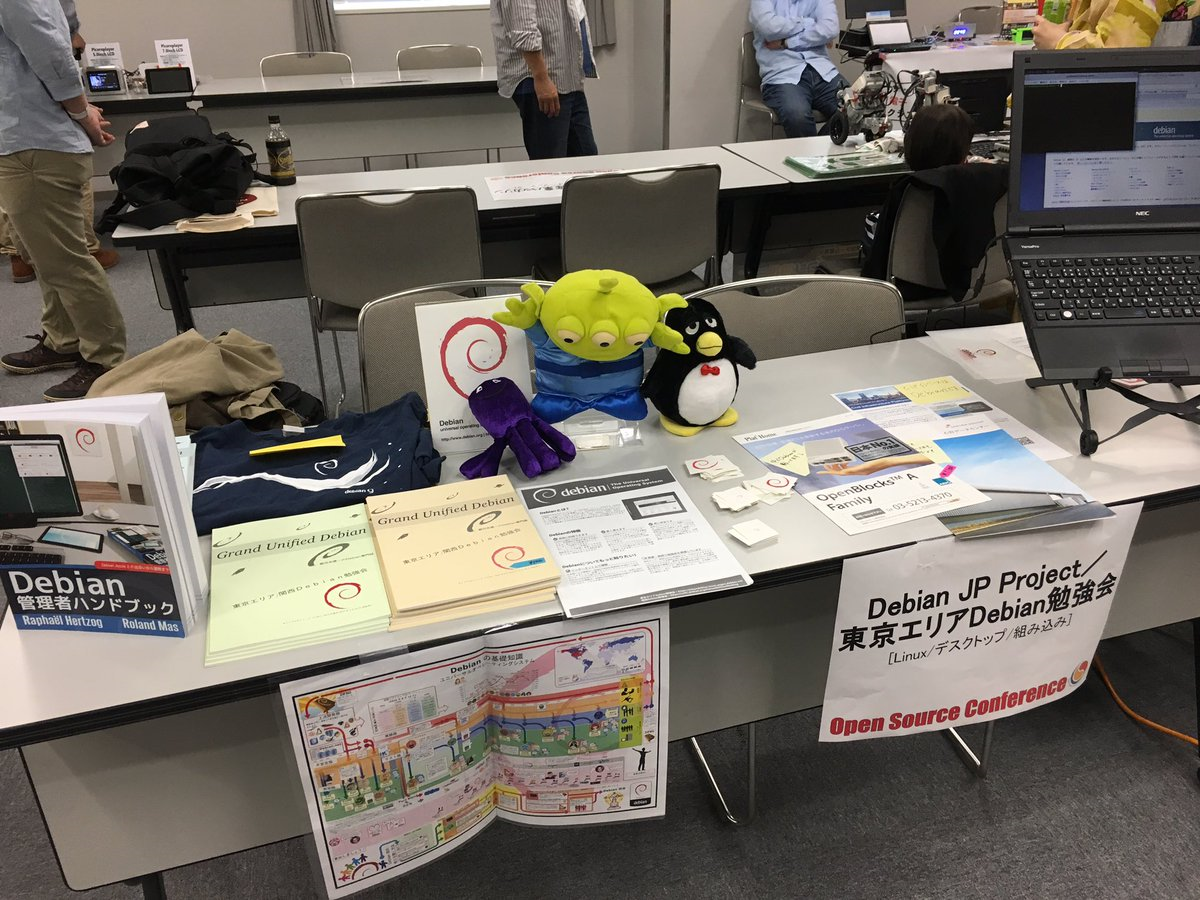
\includegraphics[width=12cm]{image201906/debianjp-booth_osc2019do.png}
    \caption{展示ブースの様子(OSC 2019 Hokkaido)}
    \label{fig:booth-osc2019do}
  \end{center}
\end{figure}

\begin{itemize}
\item ブース来訪者
  \begin{itemize}
  \item 合計 約 61 名
  \item 属性
    \begin{itemize}
    \item 男性・大人     30 名
    \item 女性・大人      5 名
    \item 男性・学生子供 25 名
    \item 女性・学生子供  1 名
    \end{itemize}
  \end{itemize}
\end{itemize}

\begin{itemize}
\item 物販
  \begin{itemize}
  \item 本:あんどきゅめんてっどでびあん\footnote{\url{https://tokyodebian-team.pages.debian.net/undocumenteddebian.html}}
    \begin{itemize}
    \item 3 冊販売
    \end{itemize}
  \item Debian Tシャツ
    \begin{itemize}
    \item 4 着販売
    \end{itemize}
  \end{itemize}
\end{itemize}


\subsubsection{ブース来訪者との情報交換}

\begin{itemize}
\item 利用OSのアンケート
  \begin{itemize}
  \item Ubuntu     10
  \item Debian      7
  \item Raspbian    4
  \item ChromeOS    1
  \item EV3 Debian  1
  \item CentOS      1
  \end{itemize}
\end{itemize}


\subsubsection{イベントの参加者や出展者との交流}

\begin{itemize}
\item LOCAL学生部
  \begin{itemize}
  \item メンバは北海道各地に散らばっている
  \item 主にslackでコミニケーションをとっている
  \item Face to Faceで会うのはOSCとそれ以外に年に1回程度
  \item 「LOCAL Students 情報ボーイズの寄稿ノート」という本を出している\footnote{\url{https://techbookfest.org/event/tbf04/circle/14720002}}\footnote{原稿はtexで書いている模様。\url{https://github.com/hyoiutu/techbookfest_localstudents_2017}}\footnote{2冊目にあたる「LOCAL Students 情報ボーイズの寄稿ノート 2.0」を当日販売していた。}
  \end{itemize}
\end{itemize}

\begin{itemize}
\item 深町先生
  \begin{itemize}
  \item 公立千歳科学技術大学の先生
  \item FMLの開発者
  \end{itemize}
\end{itemize}


\subsection{今後のDebian開発者候補の方への呼びかけ方のディスカッション}

\subsubsection{観点}

\subsubsubsection{会いに行く・会いに来る}
  
\begin{itemize}
\item 東京圏におけるイベントと地方におけるイベントの傾向の違い
\item 高校生・高専生・専門学校生・大学生におけるイベントや勉強会の参加の壁は何か(時間、金銭、距離など)
\item 学生のいる場所へ呼んでもらう方法
\item 先生とどう知り合い、どのような情報交換をしていくとよいか
\end{itemize}

\subsubsubsection{Debian勉強会における情報提供の在り方}

\begin{itemize}
\item 取り上げる話題をどう選んでいくか
  \begin{itemize}
  \item 時事ネタ、流行りネタ、利用事例
  \item インストール
  \item アプリケーション、ミドルウェアの利用
  \item 開発環境
  \item Debianの仕組み解説
  \end{itemize}
\item Debian勉強会の資料をどのようなメディアで提供するとよいか
\item Debian勉強会のセミナーのビデオ配信(ライブまたは録画)の是非
\end{itemize}

\subsubsubsection{インターネットにおける情報提供}

\begin{itemize}
\item メーリングリスト
\item ブログ記事
\item webサイト
\end{itemize}

\subsubsubsection{イベントやセミナーにおける情報提供}

\begin{itemize}
\item セミナーのテーマに取り上げる話題の選定
  \begin{itemize}
  \item OSCでは「Debian Update」という半年間を振り返る話をすることが多い。見直すべきか?
  \end{itemize}
\item 魅力あるブース展示にするための検討
\item イベントの参加者属性を意識する
  \begin{itemize}
  \item OSCは入門者向けのイベントのため、セミナーは入門レベルの難易度に設定している
  \item より高度な知識を求める人はどのようなイベントに集まるか?また、そのイベントにDebian勉強会はどう関わるか?
  \end{itemize}
\end{itemize}

\dancersection{東京エリア Debian 勉強会課題整理}{第175回東京エリアDebian勉強会参加者}

東京エリアDebian勉強会参加者でディスカッション

\subsection{Debian勉強会やDebian界隈とOSSの関わる人とのかかわり}

東京と地方のイベントの開催傾向
\begin{itemize}
\item 東京はユーザが非常に多い
    - OSCはユーザ向けイベントの傾向あり
\item 地方はユーザも開発者も集まる
\end{itemize}
\subsection{Debianを使うきっかけ}
Debianを触るきっかけ
\begin{itemize}
\item プログラミングコンテストに参加した
\end{itemize}
Debian勉強会に参加したきっかけ
\begin{itemize}
\item twitter を見て知った(henrichさん)
\item 有名な人と話がしたい、聴きたい
\end{itemize}
\subsection{世界での開発者同士の交流状況}
DebConf18で聞いたこと
\begin{itemize}
\item 東京は毎月FaceToFaceで集まっていると話したところ、海外のDDからは羨ましいという意見があった
\item 海外のDDの人口密度が低いため、ビデオ会議やメールでやりとりするしかない環境の人は多い
\end{itemize}
\subsection{Debian開発者の育成}
パッケージ作成ハンズオンセミナーをやってみたらどうか
\begin{itemize}
\item dhの使い方
\item Debian Policyの理解講座
\end{itemize}
Debian開発者になると何がうれしいのかを他の人たちは知らないのではないか
\begin{itemize}
\item Debian開発者の権限
  \begin{itemize}
  \item 自分が普段使っているソフトをパッケージにアップロードできる
  \item  porterboxが使える(移植のため)
  \end{itemize}
\item Debian開発者のおまけな特典
  \begin{itemize}
  \item https://wiki.debian.org/MemberBenefits
  \item 例
    \begin{itemize}
      \item LWN無料で読める
      \item Steamの「portal」というゲームが一部無料
      \item gandi.netでドメインが安くとれる
      \item 就職の役に立つ?
    \end{itemize}
  \end{itemize}
\end{itemize}
\subsection{Debian勉強会とイベント参加の在り方}
参加の壁(時間、金銭、距離、心情の問題)
\begin{itemize}
\item 開催回数が多すぎて初めて参加する人から見ると心理的ハードルが高い模様
\item 遠くからの参加者をDebianJPで支援できないか
  \begin{itemize}
    \item 過去に支援していたことがあった気がする
    \item イベントで話す人に対して金銭支援してきてもらう
  \end{itemize}
\item ライフステージによって勉強会やイベントに来れなくなる
  \begin{itemize}
    \item 仕方がない面がある
    \item 若い人に対してリーチする必要あり
  \end{itemize}
\end{itemize}
学生への呼び込み
\begin{itemize}
\item 学生のいるところに呼んでもらってDebian勉強会を開催する
  \begin{itemize}
  \item 呼んでもらうにも大学生とのつながりが必要
  \item どうやるとつながることができるかのいい案が浮かばない
  \end{itemize}
\item Summer Of CodeをDebianJPや日本でできないのか
  \begin{itemize}
  \item 成果をOSCなどのイベントで発表してもらうこともできそう
  \end{itemize}
\end{itemize}
オンラインで勉強会に参加できるようにする
\begin{itemize}
\item Debian勉強会を配信してみたらどうか
  \begin{itemize}
  \item どれくらい人が見てくれるかはやってみないとわからない
  \item 初めて参加する人は質問しにくい気もする
  \item wifi経由で主催者の画面をインターネットに共有しておいて、セミナー配信する形で始めてみてはどうか
  \end{itemize}
\end{itemize}
debian勉強会で取り上げるネタ
\begin{itemize}
\item 深い話の解説話
    - 例
  \begin{itemize}
    \item initの起動の処理を読み解く
    \item AWSやGCPでのブート処理はPCとどう違うのか
  \end{itemize}
  \begin{itemize}
    \item debianは中までソースコードを読めばわかる
    \item 例のような深い話はなかなか解説もないため、やってみるといいかもしれない
  \end{itemize}
\item ネタの回し方
  \begin{itemize}
  \item OSSの記事が載っている雑誌
  \item 雑誌と同じ回し方を勉強会ですると内容が被るのよくないかもしれない
  \item debianにはdebian開発の入門の流れがあるように思える
  \end{itemize}
\item ハンズオン
    - パッケージング道場
\end{itemize}
勉強会資料の公開の仕方
\begin{itemize}
\item 現状はPDFの資料を公開している
\item googleの検索でもPDFの記事はヒットする
\item HTMLで出せればいいが、ひとまずPDFの現状でもよいのではないか
\item まずは情報を出していくことが重要
\end{itemize}
webの露出
\begin{itemize}
\item 英語で検索したほうが記事のヒットが多い
\item debianで検索しても出てこないが、ubuntuの記事が検索すると出てくる
    - ask ubuntuで検索がヒットすることが多い
\item Arch Linuxのwikiの記事の情報量はすごい
\item kernelなどのビルドまわりはGentoo Wikiが強い
\end{itemize}
メディア
\begin{itemize}
\item Software Designの記事執筆(やまねさん)
    - 大変がんばっていると思う
\end{itemize}
イベント参加
\begin{itemize}
\item ODC
    \begin{itemize}
    \item 2018年にも開催されている
    \item 出たことがないため雰囲気は不明
    \item コミュニティもセミナーは出せるため出してみたらどうか
    \end{itemize}
\item Developers Summit
    \begin{itemize}
    \item 2018年は成果を見せる場になっているように感じた
    \item 開発者のガチ発表という感じでなくなっている
    \end{itemize}
\end{itemize}
\subsection{CJK開発ネタ}
日本語環境
\begin{itemize}
\item 日本語入力環境をどう維持するか
    \begin{itemize}
    \item DebianJPでも維持する人/できる人が限られている
    \item 他のディストリビューションも人手不足の問題を抱えている
    \item 新規で作業する人/作業できる人が入ってこない状況がある
    \item 人手不足の解消案としてディストリビューション間での連携も考えた方がいいかもしれない
    \end{itemize}
\item mozc
    - 比較的新しいIMだが開発が止まっている
\item authy
    \begin{itemize}
    \item FSIJが引き受けている状況
    \item こう開発したいというリストは出ている
    \item 辞書は職人芸によりスコアリングされたものになっており難解
    \end{itemize}
\item skk
    - 日本で使っている人はいたはず
\item 辞書データ
    \begin{itemize}
    \item AI処理で利用するため整備の必要あり
    \item 辞書のライセンスの考え方
    \item 辞書づくりの作業自体がフリーであるべき派
    \item 商用版のみでも辞書があれば問題ないと考える派
    \end{itemize}
\end{itemize}
海外のIM事情
\begin{itemize}
\item 中国語
    - 入力方法は2種類
    \begin{itemize}
    \item 部首
    \item 発音(こちらが多い)
    \end{itemize}
    - IMソフト
    \begin{itemize}
      \item https://rime.im/  個人で開発したことから始まる
      \item fcitx (UIM、ibusと似た機能のソフト)
    \end{itemize}
\end{itemize}
\subsection{リモート会議を行うツール}

mumble
\begin{itemize}
\item https://packages.debian.org/ja/stretch/mumble-server
\item VoIPサーバのソフトで、音声のみ
\item ライセンスはDFSG準拠
\item 会話するサーバとクライアントソフト
\end{itemize}

WebRTC を使うソフト
\begin{itemize}
\item DFSG準拠のソフトはあるのか
\end{itemize}

nageru
\begin{itemize}
\item https://packages.debian.org/sid/video/nageru
\item 利用実績はあるか
\end{itemize}

discord
\begin{itemize}
\item 画面の共有がしやすい
\item インフラ勉強会でこれを使って開催しているらしい
\end{itemize}

slackもビデオもあったと思う
\begin{itemize}
\item やりずらい
\end{itemize}

youtube
\begin{itemize}
\item コメントが下に出てくるため見にくい、主催者に伝わりづらい
\end{itemize}

Mini Hangouts
\begin{itemize}
\item 質疑応答のログがチャットを切ると消える
\end{itemize}

spreed-webrtc
\begin{itemize}
\item https://github.com/strukturag/spreed-webrtc
\end{itemize}

\subsection{ディスカッションを終えての感想}
今後Debian勉強会をどうしていくか振り返る時間をここ数年とっていなかったので、今回はよい機会だった


%for less page
%\printindex

\newpage

\begin{center}
本資料のライセンスについて
\end{center}

\begin{fontsize}{6}{6}

本資料はフリー・ソフトウェアです。あなたは、Free Software
Foundation が公表したGNU GENERAL PUBLIC LICENSEの "バージョン2"もしくはそれ以降
が定める条項に従って本プログラムを再頒布または変更することができ
ます。

本プログラムは有用とは思いますが、頒布にあたっては、市場性及び特
定目的適合性についての暗黙の保証を含めて、いかなる保証も行ないま
せん。詳細についてはGNU GENERAL PUBLIC LICENSE をお読みください。

\end{fontsize}

\begin{center}
ソースコードについて
\end{center}

本資料のソースコードは Git を使って\url{git://anonscm.debian.org/tokyodebian/monthly-report.git}
からダウンロードできます。以下に方法を示します。

\begin{commandline}
$ git clone git://anonscm.debian.org/tokyodebian/monthly-report.git
\end{commandline}
%$

\begin{multicols}{2}
 \begin{fontsize}{6}{6}
 \begin{verbatim}
            GNU GENERAL PUBLIC LICENSE
               Version 2, June 1991

 Copyright (C) 1989, 1991 Free Software Foundation, Inc.
    51 Franklin St, Fifth Floor, Boston, MA  02110-1301  USA
 Everyone is permitted to copy and distribute verbatim copies
 of this license document, but changing it is not allowed.

                Preamble

  The licenses for most software are designed to take away your
freedom to share and change it.  By contrast, the GNU General Public
License is intended to guarantee your freedom to share and change free
software--to make sure the software is free for all its users.  This
General Public License applies to most of the Free Software
Foundation's software and to any other program whose authors commit to
using it.  (Some other Free Software Foundation software is covered by
the GNU Library General Public License instead.)  You can apply it to
your programs, too.

  When we speak of free software, we are referring to freedom, not
price.  Our General Public Licenses are designed to make sure that you
have the freedom to distribute copies of free software (and charge for
this service if you wish), that you receive source code or can get it
if you want it, that you can change the software or use pieces of it
in new free programs; and that you know you can do these things.

  To protect your rights, we need to make restrictions that forbid
anyone to deny you these rights or to ask you to surrender the rights.
These restrictions translate to certain responsibilities for you if you
distribute copies of the software, or if you modify it.

  For example, if you distribute copies of such a program, whether
gratis or for a fee, you must give the recipients all the rights that
you have.  You must make sure that they, too, receive or can get the
source code.  And you must show them these terms so they know their
rights.

  We protect your rights with two steps: (1) copyright the software, and
(2) offer you this license which gives you legal permission to copy,
distribute and/or modify the software.

  Also, for each author's protection and ours, we want to make certain
that everyone understands that there is no warranty for this free
software.  If the software is modified by someone else and passed on, we
want its recipients to know that what they have is not the original, so
that any problems introduced by others will not reflect on the original
authors' reputations.

  Finally, any free program is threatened constantly by software
patents.  We wish to avoid the danger that redistributors of a free
program will individually obtain patent licenses, in effect making the
program proprietary.  To prevent this, we have made it clear that any
patent must be licensed for everyone's free use or not licensed at all.

  The precise terms and conditions for copying, distribution and
modification follow.

            GNU GENERAL PUBLIC LICENSE
   TERMS AND CONDITIONS FOR COPYING, DISTRIBUTION AND MODIFICATION

  0. This License applies to any program or other work which contains
a notice placed by the copyright holder saying it may be distributed
under the terms of this General Public License.  The "Program", below,
refers to any such program or work, and a "work based on the Program"
means either the Program or any derivative work under copyright law:
that is to say, a work containing the Program or a portion of it,
either verbatim or with modifications and/or translated into another
language.  (Hereinafter, translation is included without limitation in
the term "modification".)  Each licensee is addressed as "you".

Activities other than copying, distribution and modification are not
covered by this License; they are outside its scope.  The act of
running the Program is not restricted, and the output from the Program
is covered only if its contents constitute a work based on the
Program (independent of having been made by running the Program).
Whether that is true depends on what the Program does.

  1. You may copy and distribute verbatim copies of the Program's
source code as you receive it, in any medium, provided that you
conspicuously and appropriately publish on each copy an appropriate
copyright notice and disclaimer of warranty; keep intact all the
notices that refer to this License and to the absence of any warranty;
and give any other recipients of the Program a copy of this License
along with the Program.

You may charge a fee for the physical act of transferring a copy, and
you may at your option offer warranty protection in exchange for a fee.

  2. You may modify your copy or copies of the Program or any portion
of it, thus forming a work based on the Program, and copy and
distribute such modifications or work under the terms of Section 1
above, provided that you also meet all of these conditions:

    a) You must cause the modified files to carry prominent notices
    stating that you changed the files and the date of any change.

    b) You must cause any work that you distribute or publish, that in
    whole or in part contains or is derived from the Program or any
    part thereof, to be licensed as a whole at no charge to all third
    parties under the terms of this License.

    c) If the modified program normally reads commands interactively
    when run, you must cause it, when started running for such
    interactive use in the most ordinary way, to print or display an
    announcement including an appropriate copyright notice and a
    notice that there is no warranty (or else, saying that you provide
    a warranty) and that users may redistribute the program under
    these conditions, and telling the user how to view a copy of this
    License.  (Exception: if the Program itself is interactive but
    does not normally print such an announcement, your work based on
    the Program is not required to print an announcement.)

These requirements apply to the modified work as a whole.  If
identifiable sections of that work are not derived from the Program,
and can be reasonably considered independent and separate works in
themselves, then this License, and its terms, do not apply to those
sections when you distribute them as separate works.  But when you
distribute the same sections as part of a whole which is a work based
on the Program, the distribution of the whole must be on the terms of
this License, whose permissions for other licensees extend to the
entire whole, and thus to each and every part regardless of who wrote it.

Thus, it is not the intent of this section to claim rights or contest
your rights to work written entirely by you; rather, the intent is to
exercise the right to control the distribution of derivative or
collective works based on the Program.

In addition, mere aggregation of another work not based on the Program
with the Program (or with a work based on the Program) on a volume of
a storage or distribution medium does not bring the other work under
the scope of this License.

  3. You may copy and distribute the Program (or a work based on it,
under Section 2) in object code or executable form under the terms of
Sections 1 and 2 above provided that you also do one of the following:

    a) Accompany it with the complete corresponding machine-readable
    source code, which must be distributed under the terms of Sections
    1 and 2 above on a medium customarily used for software interchange; or,

    b) Accompany it with a written offer, valid for at least three
    years, to give any third party, for a charge no more than your
    cost of physically performing source distribution, a complete
    machine-readable copy of the corresponding source code, to be
    distributed under the terms of Sections 1 and 2 above on a medium
    customarily used for software interchange; or,

    c) Accompany it with the information you received as to the offer
    to distribute corresponding source code.  (This alternative is
    allowed only for noncommercial distribution and only if you
    received the program in object code or executable form with such
    an offer, in accord with Subsection b above.)

The source code for a work means the preferred form of the work for
making modifications to it.  For an executable work, complete source
code means all the source code for all modules it contains, plus any
associated interface definition files, plus the scripts used to
control compilation and installation of the executable.  However, as a
special exception, the source code distributed need not include
anything that is normally distributed (in either source or binary
form) with the major components (compiler, kernel, and so on) of the
operating system on which the executable runs, unless that component
itself accompanies the executable.

If distribution of executable or object code is made by offering
access to copy from a designated place, then offering equivalent
access to copy the source code from the same place counts as
distribution of the source code, even though third parties are not
compelled to copy the source along with the object code.

  4. You may not copy, modify, sublicense, or distribute the Program
except as expressly provided under this License.  Any attempt
otherwise to copy, modify, sublicense or distribute the Program is
void, and will automatically terminate your rights under this License.
However, parties who have received copies, or rights, from you under
this License will not have their licenses terminated so long as such
parties remain in full compliance.

  5. You are not required to accept this License, since you have not
signed it.  However, nothing else grants you permission to modify or
distribute the Program or its derivative works.  These actions are
prohibited by law if you do not accept this License.  Therefore, by
modifying or distributing the Program (or any work based on the
Program), you indicate your acceptance of this License to do so, and
all its terms and conditions for copying, distributing or modifying
the Program or works based on it.

  6. Each time you redistribute the Program (or any work based on the
Program), the recipient automatically receives a license from the
original licensor to copy, distribute or modify the Program subject to
these terms and conditions.  You may not impose any further
restrictions on the recipients' exercise of the rights granted herein.
You are not responsible for enforcing compliance by third parties to
this License.

  7. If, as a consequence of a court judgment or allegation of patent
infringement or for any other reason (not limited to patent issues),
conditions are imposed on you (whether by court order, agreement or
otherwise) that contradict the conditions of this License, they do not
excuse you from the conditions of this License.  If you cannot
distribute so as to satisfy simultaneously your obligations under this
License and any other pertinent obligations, then as a consequence you
may not distribute the Program at all.  For example, if a patent
license would not permit royalty-free redistribution of the Program by
all those who receive copies directly or indirectly through you, then
the only way you could satisfy both it and this License would be to
refrain entirely from distribution of the Program.

If any portion of this section is held invalid or unenforceable under
any particular circumstance, the balance of the section is intended to
apply and the section as a whole is intended to apply in other
circumstances.

It is not the purpose of this section to induce you to infringe any
patents or other property right claims or to contest validity of any
such claims; this section has the sole purpose of protecting the
integrity of the free software distribution system, which is
implemented by public license practices.  Many people have made
generous contributions to the wide range of software distributed
through that system in reliance on consistent application of that
system; it is up to the author/donor to decide if he or she is willing
to distribute software through any other system and a licensee cannot
impose that choice.

This section is intended to make thoroughly clear what is believed to
be a consequence of the rest of this License.

  8. If the distribution and/or use of the Program is restricted in
certain countries either by patents or by copyrighted interfaces, the
original copyright holder who places the Program under this License
may add an explicit geographical distribution limitation excluding
those countries, so that distribution is permitted only in or among
countries not thus excluded.  In such case, this License incorporates
the limitation as if written in the body of this License.

  9. The Free Software Foundation may publish revised and/or new versions
of the General Public License from time to time.  Such new versions will
be similar in spirit to the present version, but may differ in detail to
address new problems or concerns.

Each version is given a distinguishing version number.  If the Program
specifies a version number of this License which applies to it and "any
later version", you have the option of following the terms and conditions
either of that version or of any later version published by the Free
Software Foundation.  If the Program does not specify a version number of
this License, you may choose any version ever published by the Free Software
Foundation.

  10. If you wish to incorporate parts of the Program into other free
programs whose distribution conditions are different, write to the author
to ask for permission.  For software which is copyrighted by the Free
Software Foundation, write to the Free Software Foundation; we sometimes
make exceptions for this.  Our decision will be guided by the two goals
of preserving the free status of all derivatives of our free software and
of promoting the sharing and reuse of software generally.

                NO WARRANTY

  11. BECAUSE THE PROGRAM IS LICENSED FREE OF CHARGE, THERE IS NO WARRANTY
FOR THE PROGRAM, TO THE EXTENT PERMITTED BY APPLICABLE LAW.  EXCEPT WHEN
OTHERWISE STATED IN WRITING THE COPYRIGHT HOLDERS AND/OR OTHER PARTIES
PROVIDE THE PROGRAM "AS IS" WITHOUT WARRANTY OF ANY KIND, EITHER EXPRESSED
OR IMPLIED, INCLUDING, BUT NOT LIMITED TO, THE IMPLIED WARRANTIES OF
MERCHANTABILITY AND FITNESS FOR A PARTICULAR PURPOSE.  THE ENTIRE RISK AS
TO THE QUALITY AND PERFORMANCE OF THE PROGRAM IS WITH YOU.  SHOULD THE
PROGRAM PROVE DEFECTIVE, YOU ASSUME THE COST OF ALL NECESSARY SERVICING,
REPAIR OR CORRECTION.

  12. IN NO EVENT UNLESS REQUIRED BY APPLICABLE LAW OR AGREED TO IN WRITING
WILL ANY COPYRIGHT HOLDER, OR ANY OTHER PARTY WHO MAY MODIFY AND/OR
REDISTRIBUTE THE PROGRAM AS PERMITTED ABOVE, BE LIABLE TO YOU FOR DAMAGES,
INCLUDING ANY GENERAL, SPECIAL, INCIDENTAL OR CONSEQUENTIAL DAMAGES ARISING
OUT OF THE USE OR INABILITY TO USE THE PROGRAM (INCLUDING BUT NOT LIMITED
TO LOSS OF DATA OR DATA BEING RENDERED INACCURATE OR LOSSES SUSTAINED BY
YOU OR THIRD PARTIES OR A FAILURE OF THE PROGRAM TO OPERATE WITH ANY OTHER
PROGRAMS), EVEN IF SUCH HOLDER OR OTHER PARTY HAS BEEN ADVISED OF THE
POSSIBILITY OF SUCH DAMAGES.

             END OF TERMS AND CONDITIONS

        How to Apply These Terms to Your New Programs

  If you develop a new program, and you want it to be of the greatest
possible use to the public, the best way to achieve this is to make it
free software which everyone can redistribute and change under these terms.

  To do so, attach the following notices to the program.  It is safest
to attach them to the start of each source file to most effectively
convey the exclusion of warranty; and each file should have at least
the "copyright" line and a pointer to where the full notice is found.

    <one line to give the program's name and a brief idea of what it does.>
    Copyright (C) <year>  <name of author>

    This program is free software; you can redistribute it and/or modify
    it under the terms of the GNU General Public License as published by
    the Free Software Foundation; either version 2 of the License, or
    (at your option) any later version.

    This program is distributed in the hope that it will be useful,
    but WITHOUT ANY WARRANTY; without even the implied warranty of
    MERCHANTABILITY or FITNESS FOR A PARTICULAR PURPOSE.  See the
    GNU General Public License for more details.

    You should have received a copy of the GNU General Public License
    along with this program; if not, write to the Free Software
    Foundation, Inc., 51 Franklin St, Fifth Floor, Boston, MA  02110-1301 USA


Also add information on how to contact you by electronic and paper mail.

If the program is interactive, make it output a short notice like this
when it starts in an interactive mode:

    Gnomovision version 69, Copyright (C) year  name of author
    Gnomovision comes with ABSOLUTELY NO WARRANTY; for details type `show w'.
    This is free software, and you are welcome to redistribute it
    under certain conditions; type `show c' for details.

The hypothetical commands `show w' and `show c' should show the appropriate
parts of the General Public License.  Of course, the commands you use may
be called something other than `show w' and `show c'; they could even be
mouse-clicks or menu items--whatever suits your program.

You should also get your employer (if you work as a programmer) or your
school, if any, to sign a "copyright disclaimer" for the program, if
necessary.  Here is a sample; alter the names:

  Yoyodyne, Inc., hereby disclaims all copyright interest in the program
  `Gnomovision' (which makes passes at compilers) written by James Hacker.

  <signature of Ty Coon>, 1 April 1989
  Ty Coon, President of Vice

This General Public License does not permit incorporating your program into
proprietary programs.  If your program is a subroutine library, you may
consider it more useful to permit linking proprietary applications with the
library.  If this is what you want to do, use the GNU Library General
Public License instead of this License.
 \end{verbatim}
 \end{fontsize}
\end{multicols}

\begin{center}
Debian オープンユーズロゴ ライセンス
\end{center}

\begin{multicols}{2}
 \begin{fontsize}{6}{6}
 \begin{verbatim}

Copyright (c) 1999 Software in the Public Interest
Permission is hereby granted, free of charge, to any person
obtaining a copy of this software and associated documentation
files (the "Software"), to deal in the Software without restriction,
including without limitation the rights to use, copy, modify, merge,
publish, distribute, sublicense, and/or sell copies of the Software,
and to permit persons to whom the Software is furnished to do so,
subject to the following conditions:

The above copyright notice and this permission notice shall be
included in all copies or substantial portions of the Software.

THE SOFTWARE IS PROVIDED "AS IS", WITHOUT WARRANTY OF ANY
KIND, EXPRESS OR IMPLIED, INCLUDING BUT NOT LIMITED TO THE
WARRANTIES OF MERCHANTABILITY, FITNESS FOR A PARTICULAR PURPOSE AND
NONINFRINGEMENT. IN NO EVENT SHALL THE AUTHORS OR COPYRIGHT HOLDERS
BE LIABLE FOR ANY CLAIM, DAMAGES OR OTHER LIABILITY, WHETHER IN
AN ACTION OF CONTRACT, TORT OR OTHERWISE, ARISING FROM, OUT OF OR
IN CONNECTION WITH THE SOFTWARE OR THE USE OR OTHER DEALINGS IN
THE SOFTWARE.
 \end{verbatim}
 \end{fontsize}
\end{multicols}

% 問題と回答が同じみひらきにならないようにする
%\cleartoevenpage
%-------------------------------------------------------------------------------
%\dancersection{Debian Trivia Quiz 問題回答}{}
%-------------------------------------------------------------------------------

 Debian Trivia Quiz の問題回答です。
 あなたは何問わかりましたか? \\
 %回答はdebianmeetingresume2014-fuyu.jqzというファイルに生成されるので、
 %それを手動でコピペして使う。
 % ここからコピペ
 % FIXME 問題が全部はいったらコピペすること
 %(progn (next-line 1)(insert-file "debianmeetingresume2013-fuyu.jqz") )
%\begin{enumerate}
%\end{enumerate}

% add page to even number
%\newpage
\cleartooddpage

\newpage
\thispagestyle{empty}\mbox{}
\newpage

\thispagestyle{empty}
{
\large
\begin{itembox}{\bf 『あんどきゅめんてっど でびあん』について}
本書は、東京および関西周辺で毎月行なわれている『東京エリア Debian 勉強会』および
『関西 Debian 勉強会』で
使用された資料・小ネタ・必殺技などを一冊にまとめたものです。
% FIXME: 範囲を修正すること。
収録範囲は2019/07〜2019/11まで
内容は無保証、つっこみなどがあれば勉強会にて。
\end{itembox}
}

\vspace*{16cm}
{\color{dancerlightblue}\rule{\hsize}{1mm}}
\vspace{2mm}

\includegraphics[width=2cm]{image200502/openlogo-nd.eps}
\noindent \Large \bf あんどきゅめんてっど でびあん 2019年冬号\\
\noindent \normalfont 2019年12月31日 \hspace{5mm}  初版第1刷発行\\
\noindent \normalfont 東京エリア Debian 勉強会/関西Debian 勉強会 (編集・印刷・発行)\\
{\color{dancerdarkblue}\rule{\hsize}{1mm}}

\end{document}
